%5 
%bib done
%examples
%tables
%crossrefs

 
\section{Introduction}\label{sec:5:1}


\hypertarget{Toc376958238}{}
 

One approaches the study of kinship\is{kinship} in Eastern Indonesia with some trepidation, for it has a chequered past. For a time Eastern Indonesia and especially East Nusantara was a nexus of kinship studies \citep[see][]{Fox1980,VanWouden1968}. Within linguistics a comparative approach tackled issues of the reconstruction of the proto-Austronesian\il{proto-Austronesian} kinship system and sought to understand how kinship can inform our knowledge of culture history. At the same time the study of kinship was losing its favored place in anthropological theory, as authors such as \citet{Schneider1984} argued that the notion of kinship itself should be considered a cultural construct, not necessarily universal. While these academic trends had notably less effect on the Dutch school prevalent in Indonesian kinship studies, there has nonetheless been relatively little work on kinship in the region over the past two decades, and almost none in Alor-Pantar. More recently, a renewed interest in symbolic meaning has brought anthropological and linguistic approaches more closely in line \citep[see][]{Schweitzer2000}. Without revisiting the anthropological debates that have shaped the study of kinship, this chapter takes a more traditional approach to kinship, focusing first and foremost on kinship terminology. Kinship as practice may well be a cultural construct, but it is necessarily grounded in a web of linguistic terminological structure. This chapter can be read as a first step toward understanding that terminology in the Alor-Pantar languages within a comparative context.

The kinship systems in Alor-Pantar languages exhibit great variation. The westernmost languages, Blagar\il{Blagar}, Teiwa\il{Teiwa}, and Western Pantar\il{Western Pantar}, classify siblings and parallel cousins together in distinction to cross-cousins. That is, children of same-sex siblings (parallel cousins) are classified using the same terminology as used for siblings, while children of opposite-sex siblings (cross-cousins) are classified using distinct terminology. Marriage between cross-cousins is or was until recently considered the ideal. At the opposite extreme, in the highlands of Alor, Kamang\il{Kamang} expressly forbids cross-cousin marriage. Other languages show traces of asymmetrical exchange, reflected either in their kinship terminologies, in their marriage practices, or both. These languages distinguish the relationship between a man and his female maternal cross-cousin, his mother's brother's daughter, but do not highlight the relationship between a man and his paternal female cross-cousin. Even among languages whose kinship systems are roughly similar, the terms themselves are often not cognate. Likewise, cognate terms often have varying semantics across the languages. The general picture which emerges is one of drift toward symmetric exchange. Several independent sub-patterns can be identified. These will be discussed following a description of the systems in each of the individual languages.

An important aspect of all the kinship systems considered here is the identification of cross-cousins. Children of same-sex siblings are classed as siblings, whereas children of opposite-sex siblings are cross-cousins and in some languages are considered ideal marriage partners. While this basic distinction is preserved to a greater or lesser degree across the languages, there is significant variation in kinship terminologies. Comparing these systems provides insight into the history and dispersal of the Alor-Pantar languages, as well as possible language contact scenarios.

In this chapter I compare kinship terminology in eight Alor-Pantar languages forming a broad geographic and typological sample of the family (see the Sources section at the end of this chapter for details). For all of the languages, data were obtained by eliciting genealogies for several individuals and then discussing those genealogies with both the same and other individuals in order to verify and fill in any gaps in the systems. For Western Pantar\il{Western Pantar} I relied also on my own fieldnotes from several years of work with the language, and for Blagar\il{Blagar} I also drew on the description in \citet{Steinhauer1993}. For those two languages the kinship terminology can be considered complete. For the remaining languages it is possible that some terms have been overlooked. Hence, the absence here of, say, a Teiwa\il{Teiwa} term by which the wives of two brothers address each other should not be taken as evidence that such a term does not exist in Teiwa\il{Teiwa}. It is possible that such a term does exist but has not yet been recorded.

The following section describes the kinship\is{kinship} terminology in each of the eight languages individually. Then in {\SS} \ref{sec:5:3} these terminologies are compared across the languages. {\SS} \ref{sec:5:4} presents a brief description of marriage prescriptions. Finally, {\SS} \ref{sec:5:5} concludes with a discussion of the likely history of kinship systems in the Alor-Pantar languages. 


\section{Kin terminology}\label{sec:5:2}
In the following subsections the inventory of kinship\is{kinship} terminology is described for each of the eight languages in the sample. The descriptions begin with terminology in ego's generation and then proceeds to ascending generations, descending generations, and finally affines (kin related by marriage). A summary table of kinship terms for each language is found at the end of each subsection.\footnote{Abbreviations used for kin type primitives are as follows: mother [M], father [F], sister [Z], brother [B], daughter [D], son [S], child [C], husband [H], wife [W], man speaking [m], woman speaking [f], elder [e], younger [y].}   Since most kinship terms are obligatorily possessed in Alor-Pantar languages, the terms are cited here as bound morphemes. Full forms inflected for first-person can be derived by adding the first-person singular prefix, which is composed of an alveolar nasal plus a vowel whose quality varies by language (\textit{n-}/\textit{na-}/\textit{no-}/\textit{ne-}). Thus, Western Pantar \textit{-iar} `father'; \textit{niar} `my father'.

\subsection{Western Pantar}\label{sect_wp}
Western Pantar\il{Western Pantar} has the most elaborated set of sibling/cousin terms of any language described here. A single terminology for siblings and parallel cousins includes five terms distinguished by age and relative gender (see Table \ref{tab:5:table_wp_terms} at the end of this section). Same-sex elder siblings are distinguished for gender, while same-sex younger siblings are not distinguished for gender. Opposite-sex siblings are not distinguished for age. The formal similarity between the form \textit{-aipang} `man's sister' and \textit{-aiyang} `woman's brother' is probably not accidental. These terms likely derive from the possessive\is{possession} pronoun\is{pronoun} formative \textit{ai} (cf. \textit{nai} `mine', \textit{gai} `his/her') plus \textit{pang} `non-marriageable of ego's generation' and \textit{yang} `return from above'. So a man's sister is ``that of mine which is non-marriageable''; while a woman's brother is ``that of mine which descends from above'', i.e., that which comes down from my descent group. 

Children of same-sex siblings are classed as siblings, whereas children of opposite-sex siblings are cross-cousins. The same-sex cross-cousin terms in Western Pantar\il{Western Pantar} are mutually exclusive; that is, there is no general cross-cousin term which subsumes the others. Thus, \textit{-'ar} `man's male cross-cousin' and \textit{-ingtamme} `woman's female cross-cousin' refer only to same-sex, non-marriageable cross-cousins. In contrast, the term for opposite-sex cross-cousin is independent of the gender of the ego and referent. The term \textit{baddang} `opposite-sex cross-cousin' is often described as meaning `marriageable' and represents the closest marriageable relationship, often said to be the ideal marriage. The terminology in ego's generation thus differs according to whether the ego is female (Figure \ref{fig:5:1}) or male (Figure \ref{fig:5:2}).

\begin{figure}[b]
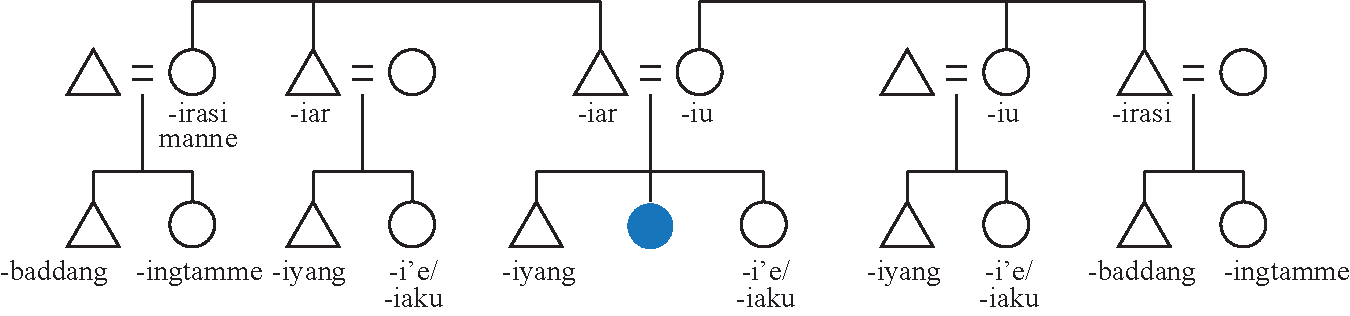
\includegraphics[width=\textwidth]{figures/Holton_ch5_fig1.pdf}
%\includegraphics[width=6.2665in,height=1.9146in,width=\textwidth]{fc7457c206664b669ab0bf2a407db9b7-img1}
\caption{Western Pantar\ilt{Western Pantar} terminology in ego's and ascending generation (female ego)}
\label{fig:5:1}
\end{figure}  
 
\begin{figure}[t]
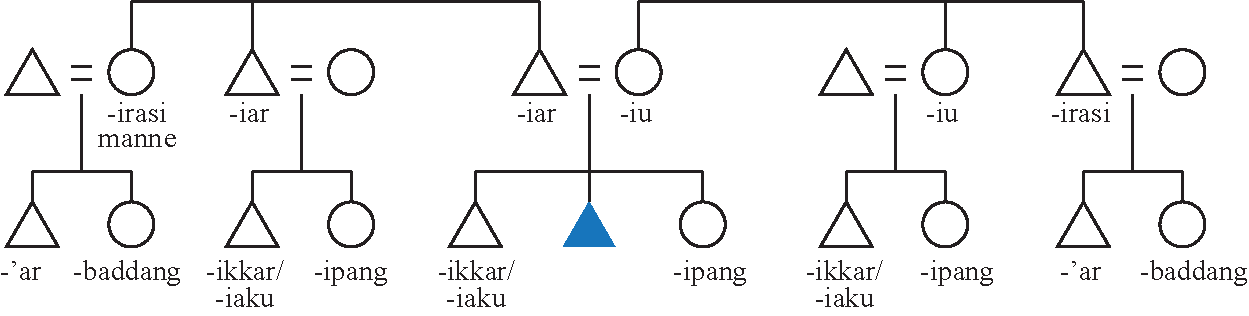
\includegraphics[width=\textwidth]{figures/Holton_ch5_fig2.pdf}
% \includegraphics[width=6.2665in,height=1.9146in,width=\textwidth]{fc7457c206664b669ab0bf2a407db9b7-img2} 
\caption{Western Pantar terminology in ego's and ascending generation (male ego)}
\label{fig:5:2}
\end{figure} 
 

The term \textit{-ai tane} is synonymous with \textit{baddang,} though it is not used as a vocative\textit{.} This term likely derives from an archaic word \textit{ne} `body' with a fossilized distributive possessive\is{possession} prefix \textit{ta}. It is possessed using the alienable\is{alienability} possessive\is{possession} paradigm, thus, \textit{nai tane} `my marriageable cross-cousin', or more literally, `that of our body'. Marriageable cross-cousins may also be referred to (though not addressed) by the term \textit{wallang}, a more general term which refers to the entire mother's brother's or father's sister's descent group, including the marriageable cross-cousins. The term \textit{wallang} contrasts with \textit{pang}, which refers to ego's own descent group. The exchange of women from one's own descent group to one's \textit{wallang} is highlighted in the common expression \textit{pang wallang gar da'ai} `one from our clan shared with the opposite clan', a figurative reference to a woman who marries outside the clan. 

 
There is some skewing of terms in the first ascending generation. Same-sex siblings of one's parents are classed as parents, but there is no entirely separate term distinguishing father's sister from mother's brother. Mother's brother is \textit{-irasi} (vocative \textit{dasi}). Father's sister can also be referred to as \textit{-irasi} but is more likely to be called by the modified term \textit{-irasi manne} or \textit{-irasi eu} (cf. \textit{manne} `wife', \textit{eu} `woman'). These latter terms can also denote the spouse of \textit{-irasi}, while the spouse of \textit{-irasi manne} is \textit{-irasi ammu} (\textit{ammu} `man') or simply \textit{-irasi.} The descending term \textit{-airas} refers to children of one's opposite-sex siblings. Thus, \textit{-irasi} and \textit{-airas} are reciprocal terms. In Steinhauer's (1993) formulation \textit{-irasi} and \textit{-airas} denote potential parents-in-law and potential children-in-law, respectively. Indeed, these terms are used for affines as well, using the equations MB = WF and FZ = WM, characteristic of a symmetric system of marriage alliance (see {\SS} \ref{sec:5:4}). That is, one's spouse's parents are denoted by the same terms used for one's parent's opposite-sex siblings, since ideally one's spouse would be the offspring of one's parent's opposite-sex sibling, i.e., a cross-cousin. 

  A crucial aspect of the Western Pantar\il{Western Pantar} kinship\is{kinship} system is that all marriages are treated as if they were marriages between cross-cousins, even when they are not. Thus, if I marry a woman who is not my \textit{-baddang}, I assume relationships to her kin as if she were my cross-cousin. In particular, I refer to her parents as \textit{nirasi}, while they refer to me as \textit{nairas.} So, affine terminology can to a large part be derived from the consanguine terminology with the assumption of cross-cousin marriage (see Figure \ref{fig:5:3}).


\begin{figure}[t]
\centering
%\includegraphics[width=1.7728in,height=1.5701in,width=\textwidth]{fc7457c206664b669ab0bf2a407db9b7-img3}
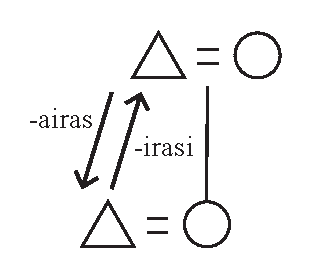
\includegraphics[width=4.5cm]{figures/Holton_ch5_fig3.pdf}
\caption{ Western Pantar\ilt{Western Pantar} affine relations in ascending and descending generation. Terms are independent of gender of ego or referent.}
\label{fig:5:3}
\end{figure}  


\begin{figure}
\centering
%\includegraphics[width=3.2728in,height=2.4866in,width=\textwidth]{fc7457c206664b669ab0bf2a407db9b7-img4}
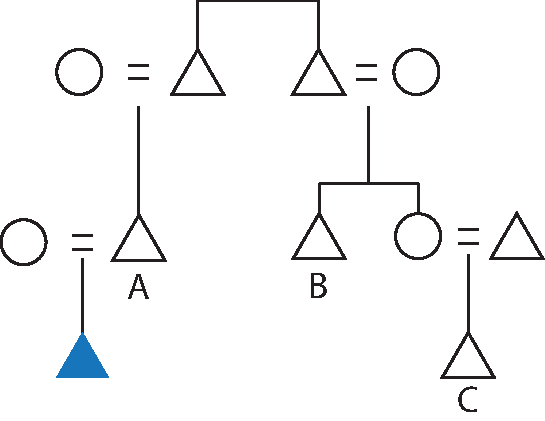
\includegraphics[width=6.5cm]{figures/Holton_ch5_fig4.pdf}
\caption{More distant kin relations in Western Pantar\ilt{Western Pantar}. Ego calls C \textit{na'ar} `man's male cross-cousin'}
\label{fig:5:4}
\end{figure}   

Moreover, some rather distant relationships can appear quite close. For example, in Figure \ref{fig:5:4} the relationship between ego and C is one of cross-cousins; that is, ego calls C \textit{na'ar.} This is true even though the biological parents of ego and C are not biological siblings. The key here is that the parents of ego and C are indeed classificatory siblings. This is because A and B, as children of same-sex siblings, are themselves classificatory siblings, hence B's sister, who is also C's mother, must also be sister to A. 


The genetic distance between relationships such as those in Figure \ref{fig:5:4} does not go unnoticed, particularly with respect to the opposite-sex sibling terms \textit{-ipang} `man's sister' and \textit{-iyang} `woman's brother'. The word \textit{haila} `base, main, area' can be used to indicate a relationship which is perceived to be biologically closer. Thus, \textit{-ipang haila} `man's sister, closely related' and \textit{-iyang haila} `woman's brother, closely related'. The terms containing \textit{haila} do not necessarily indicate biological siblings but are mainly contrastive in usage, indicating a closer relationship. The use of \textit{haila} is based on the metaphor \textit{yattu haila}, denoting the area underneath the branches of a tree (\textit{yattu} `tree').

Affine terminology in ego's generation is derived from sibling terminology, qualified with the gender terms \textit{manne} `female' and \textit{ammu} `male'. The choice of sibling term indicates the relationship either between ego and ego's sibling or between ego's spouse and ego's spouse's sibling. The gender qualifiers are used to indicate the gender of the referent for affine terms. Thus, \textit{-i'e} occurs in constructions referring to `woman's older sister', `man's wife's elder sister' (\textit{-i'e manne}), and `woman's elder sister's husband' (\textit{-i'e ammu}). Since younger siblings are not differentiated by ego's gender, the affine terms derived from \textit{-iaku} `younger sibling' are synonymous between spouse's sibling and sibling's spouse.

There is a paucity of Western Pantar\il{Western Pantar} terms referring to generations two or more removed from ego. The terms \textit{kuba} `old woman' and \textit{wenang} `old man' can be used vocatively for `grandmother' and `grandfather', respectively. These terms can also be used to derive polite forms of address for one's paternal grandparents, namely, \textit{manne kuba} `father's mother' (literally, `female old woman') and \textit{-ikkar wenang} `father's father' (literally, `man's elder brother old man'). The terms \textit{kuba} and \textit{wenang} can also be used referentially in conjunction with a possessive\is{possession} pronoun\is{pronoun}, though the reference need not be restricted to persons of the second generation above ego.




\begin{table}
\centering
\footnotesize
%
% it ain't pretty, but using footnotesize at least allows this table to fit on a single page
%
\begin{tabular}{p{2.5cm}L{3cm}L{5.5cm}}
\mytopline
\textit{{}-iar} & F, FB & father, paternal uncle\\
\textit{{}-iu} & M, MZ & mother, maternal aunt\\
\textit{{}-irasi} & MB, MZH, WF, WM, HM, HF & maternal uncle\\
\textit{{}-irasi manne}

\textit{{}-irasi eu} & FZ, MBW & paternal aunt (lit. `female uncle')\\
\textit{{}-irasi (ammu)} & FZH & paternal aunt's wife\\
\textit{{}-airas} & mZC, fBC, WBC, HZC, CW, CH & child of opposite-sex sibling\\
\textit{{}-ikkar} & meB & man's elder brother\\
\textit{{}-i'e} & feZ & woman's elder sister\\
\textit{{}-iaku} & myB, fyZ & younger same-sex sibling\\
\textit{{}-aipang} & mZ & man's sister\\
\textit{{}-aiyang} & fB & woman's brother\\
\textit{{}-ingtamme} & fMBD, fFZD & woman's same-sex cross-cousin\\
\textit{{}-'ar} & mMBS, mFZS & man's same-sex cross-cousin\\
\textit{{}-baddang} / \newline \-\hspace{.1cm} \textit{wallang} / \newline \-\hspace{.1cm} \textit{{}-ai tane} & fMBS, fFZS, mMBD, mFZD & opposite-sex cross-cousin, \newline \-\hspace{.1cm} opposite clan (marriageable)\\
\textit{pang} &  & same clan (non-marriageable)\\
\textit{{}-imu} & H & husband\\
\textit{{}-ru} & W & wife\\
\textit{{}-ikkar ammu} & HeB & woman's husband's elder brother \newline \-\hspace{.1cm} (lit. `male elder brother')\\
\textit{{}-ikkar manne} & meBW & man's elder brother's wife \newline  \-\hspace{.1cm} (lit. `female elder brother')\\
\textit{{}-i'e ammu} & feZH & woman's elder sister's husband \newline \-\hspace{.1cm} (lit. `male elder sister')\\
\textit{{}-i'e manne} & WeZ & man's wife's elder sister \newline \-\hspace{.1cm} (lit. `female elder sister')\\
\textit{-iaku ammu} & HyB, fyZH & husband's younger brother, woman's younger sister's husband \newline \-\hspace{.1cm} (lit. `male younger sibling')\\
\textit{{}-iaku manne} & WyZ, myBW & wife's younger sister, man's younger brother's wife  \newline \-\hspace{.1cm} (lit. `female younger sibling')\\
\textit{wenang} & FF, MF & grandfather\\
\textit{{}-ikkar wenang} & FF & paternal grandfather (lit. `grandfather elder brother')\\
\textit{kuba} & FM, MM & grandmother\\
\textit{manne kuba} & FM & paternal grandmother (lit. `female grandmother')\\
\textit{{}-wake} & C, mBC, fZC & child, child of same-sex sibling\\
\textit{{}-wake ammu} & S, mBS, fZS & son (lit. `male child')\\
\textit{{}-wake eu} & D, mBD, fZD & daughter (lit. `female child')\\
\mybottomline
\end{tabular}

\caption{Western Pantar\ilt{Western Pantar} kinship\ist{kinship} terms}
\label{tab:5:table_wp_terms}
\end{table}
 
 \newpage
 
\subsection{Teiwa}\label{sect_teiwa}
\label{bkm:Ref247777020}In Teiwa\il{Teiwa}, as in many of the AP languages, there are two sets of sibling terminologies with a certain amount of overlap in usage (See Table~\ref{tab:5:teiwakin} at the end of this section). The first is gender-based, distinguishing \textit{-gasqai} `classificatory sister' and \textit{-ianqai} `classificatory brother'. These terms include both siblings and parallel cousins. These terms are evidently bimorphemic, as the second contrasts with \textit{-ian} `cross-cousin'. The second morpheme \textit{qai} may possibly be related to \textit{qai} `only' or \textit{-oqai} `child'. The form \textit{-gas} on its own has no meaning. A second set of sibling terminology is age-based, distinguishing \textit{-ka'au} `elder sibling' and \textit{-bif}  `younger sibling'. There is a strong preference for using the age-based terminology with same-sex siblings and using the gender-based terminology with opposite-sex siblings, but this preference does not form a strict division between the two terminologies. 

Cross-cousins are not referred to by either of these terminologies but instead by the term \textit{-ian}. Opposite-sex cross-cousins, i.e., marriageable cross-cousins, are referred to as  \textit{-dias}. In contrast to Western Pantar\il{Western Pantar}, cross-cousin terminology does not distinguish the gender of either the ego or the referent (see Figures \ref{fig:5:5} and \ref{fig:5:6}).

\begin{figure}[h]
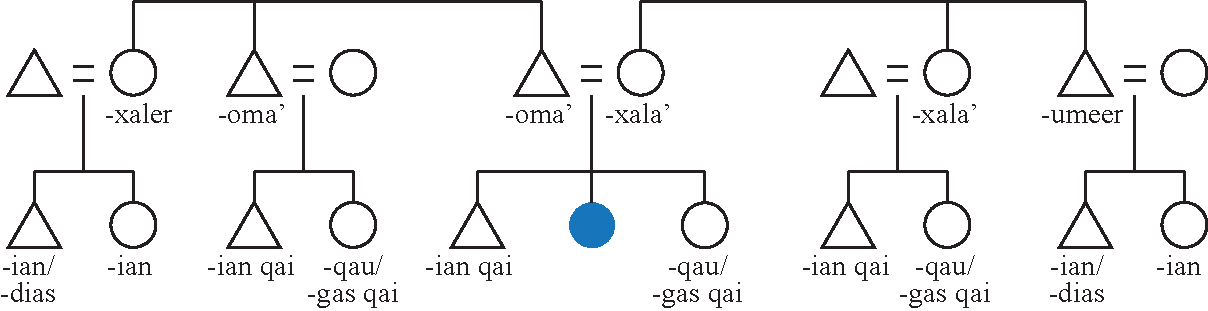
\includegraphics[width=\textwidth]{figures/Holton_ch5_fig5.pdf}
%\includegraphics[width=6.2583in,height=1.9165in,width=\textwidth]{fc7457c206664b669ab0bf2a407db9b7-img5}
\caption{Teiwa terminology in ego's and ascending generation (female ego). }
\label{fig:5:5}
\end{figure}   

\begin{figure}[b]
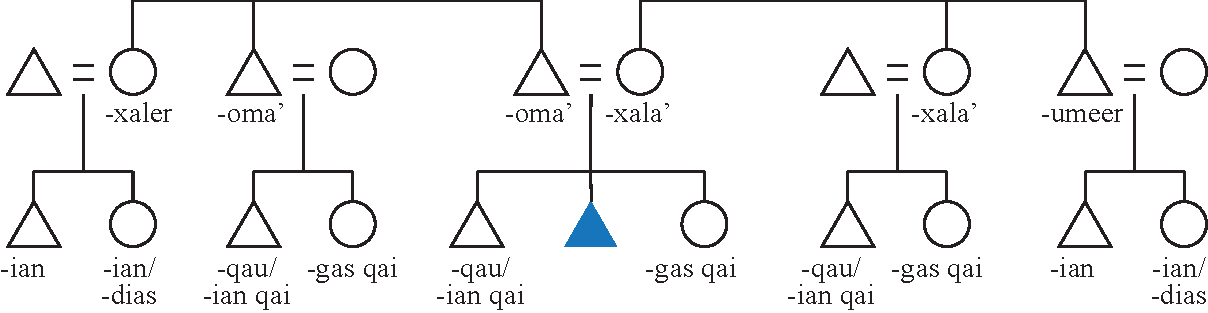
\includegraphics[width=\textwidth]{figures/Holton_ch5_fig6.pdf}
 %\includegraphics[width=6.2583in,height=1.9165in,width=\textwidth]{fc7457c206664b669ab0bf2a407db9b7-img6}
\caption{Teiwa terminology in ego's and ascending generation (male ego) }
\label{fig:5:6}
\end{figure}  
 

Marriageable cross-cousins can also be referred to as \textit{-bruman yis,} though this term is not used as a term of address. The term \textit{-bruman} itself indicates `marriageable one' and may have been borrowed from neighboring Blagar\il{Blagar} \textit{-boromung}, which is the sole term for marriageable cross-cousin in that language. The qualifier \textit{yis} denotes `fruit'. In Teiwa\il{Teiwa} the unqualified term \textit{-bruman} is not necessarily restricted to children of one's parent's opposite-sex sibling, but may apply more broadly. Preference for cross-cousin marriage remains strong in Teiwa\il{Teiwa}, and marriages which fail to meet this criteria -- that is, marriages not to one who is in the `marriageable' category denoted by \textit{bruman}{} -- are not as readily integrated into the kinship system as they are in Western Pantar\il{Western Pantar}. As in Western Pantar\il{Western Pantar} marriages are treated as if they obeyed cross-cousin rules, even when they don't. Thus, one refers to the sibling of one's sibling's spouse as a cross-cousin, for had one's sibling married their cross-cousin, that person would be one's cross-cousin as well. However, in Teiwa\il{Teiwa}, when a same-sex sibling marries a non cross-cousin, speakers express reluctance to call this sibling's spouse (fZH, mBW) by the term \textit{-dias}, since in some sense this person is not really a cross-cousin. This is avoided by using the more general cross-cousin term \textit{-ian}, or simply by addressing the sibling's spouse as \textit{-gasqai} `sister'. 

The Teiwa kinship\is{kinship} system contains the largest inventory of mono-morphemic terms relating to cross-cousins of any of the eight languages discussed here. Uniquely, it has distinct mono-morphemic terms referring to father's sister \textit{-xaler} and mother's brother \textit{-umeer}. In the other languages one or more of these terms is derived. In Western Pantar\il{Western Pantar} the term FZ is derived from MB ({\SS} \ref{sect_wp}); in Blagar\il{Blagar} the terms MB and FZ are derived from F and M, respectively ({\SS} \ref{sect_blagar}). In terms of both structure and practice the Teiwa exhibits an extremely symmetrical system, with equal distinction given to the father's sister and mother's brother. 

As in Western Pantar\il{Western Pantar}, affines in ego's generation employ the same terms as used for cross-cousins. The spouse of one's opposite-sex sibling is referred to as \textit{-ian}, while the spouse of one's same-sex sibling is referred to as \textit{-dias.} Affines in the descending generation are denoted \textit{-rat}, regardless of gender, while affines in the ascending generation are denoted by the same terms used for mother's brother and father's sister, namely \textit{-umeer} or \textit{-xaler}. 

Many Teiwa kinship terms can be further modified for relative age. All of the ascending terms can be modified with \textit{uwaad} `big' and \textit{sam} `small' to indicate relatively older or younger age, respectively (these modifiers are omitted from Figure \ref{fig:5:5} and Figure \ref{fig:5:6} above); thus, \textit{numeer uwaad} `my mother's elder brother'. The terms in ego's generation can be modified with \textit{matu} `eldest', \textit{bak} `middle', and \textit{iik} `youngest'.  Terms which are not already specified for gender can be optionally specified with \textit{eqar} `female' or \textit{masar} `male'; thus, \textit{noqai eqar} `my daughter'.\enlargethispage{1em}




\begin{table}
\begin{tabular}{llL{5cm}}
\mytopline
\textit{{}-oma'} & F, FB & father, paternal uncle\\
\textit{{}-xala'} & M, MZ & mother, maternal aunt\\
\textit{{}-umeer} & MB, FZH, WF, HF & maternal uncle\\
\textit{{}-xaler} & FZ, MBW, HM, WM & paternal aunt\\
\textit{{}-gasqai} & Z, MZD, FBD & sister, female parallel cousin\\
\textit{{}-ianqai} & B, MZS, FBS & brother, male parallel cousin\\
\textit{{}-ka'au} & eB, eZ, MeZC, FeBC & elder sibling, parallel cousin via parent's younger sibling\\
\textit{{}-bif} & yB, yZ, MyZC, FyBC & younger sibling, parallel cousin via parent's elder sibling\\
\textit{{}-ian} & MBC, FZC & cross-cousin\\
\textit{{}-dias} & fMBS, fFZS, mMBD, mFZD & opposite-sex cross-cousin\\
\textit{{}-bruman yis} & fMBS, fFZS, mMBD, mFZD & opposite-sex cross-cousin\\
\textit{{}-misi} & H & husband\\
\textit{{}-emaq} & W & wife\\
\textit{{}-rat} & mZC, fBC, SW, DH & affine of descending generation\\
\textit{{}-rat masar} & DH & son-in-law (lit. `male affine')\\
\textit{{}-rat eqar} & SW & daughter-in-law (lit. `female affine')\\
\textit{{}-rat emaq} & fBD, mZD, WBD, SW & daughter-in-law, daughter of opposite-sex sibling\\
\textit{{}-oqai} & C & child\\
\textit{{}-rata'} & FF, FM, MF, MM & grandparent\\
\textit{{}-rat qai} & CC & grandchild\\
\mybottomline
\end{tabular}

\caption{Teiwa\ilt{Teiwa} kinship\ist{kinship} terms}
\label{tab:5:teiwakin}
\end{table}

\clearpage
\subsection{Blagar}\label{sect_blagar}\ilt{Blagar}
Blagar employs a single set of gender-based terminology for classificatory siblings (siblings and parallel cousins) which distinguishes \textit{-kaku} `same-sex sibling' and \textit{-edi} `opposite-sex sibling'. Cross-cousins are distinguished by the term \textit{-ebheang}. Additionally, cross-cousins of the opposite-sex may be optionally referred to as \textit{-boromung}. Like its Teiwa\il{Teiwa} cognate \textit{-bruman}, the term \textit{-boromung} distinguishes marriageable cross-cousins, or what Steinhauer refers to as ``potential spouses''. However, this term is avoided in the presence of the referent, in which case \textit{-ebheang} is preferred \citep[156]{Steinhauer1993}. The term \textit{-ebheang} refers to all cross-cousins, regardless of the gender of ego or referent.


\begin{figure}[h]
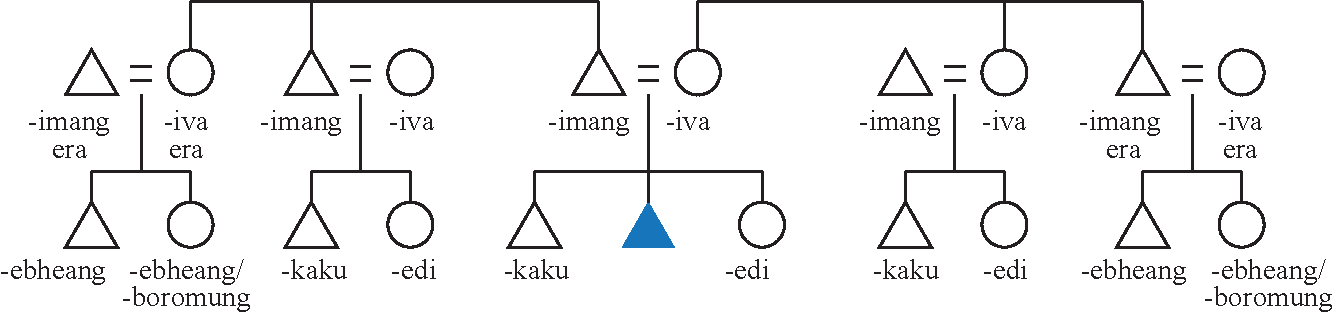
\includegraphics[width=\textwidth]{figures/Holton_ch5_fig7.pdf}
 %\includegraphics[width=6.2583in,height=1.9165in,width=\textwidth]{fc7457c206664b669ab0bf2a407db9b7-img7}
\caption{Blagar terminology in ego's and ascending generation (male ego) }
\label{fig:5:7}
\end{figure}  
 

 

The parents of ego's cross-cousins -- i.e., ego's father's sister and her husband, and ego's mother's brother and his wife -- are distinguished by compounding the classificatory mother and father terms with \textit{era} `base'. The reciprocal relationship is indicated by \textit{-bhilang.} This terminology changes when cross-cousin marriages are actually realized. If ego marries his or her cross-cousin, then ego's \textit{-imang era} and \textit{-iva era} become simply \textit{-idat} `in-laws'. Similarly, these new parents-in-law now also refer to ego as \textit{-idat} rather than \textit{-bhilang}, so that \textit{-idat} is its own reciprocal. Affines in ego's generation are denoted \textit{-des}, though this term is usually restricted to same-sex referents.\footnote{The term \textit{-des} is not reported for the Dolap dialect described by \citet{Steinhauer1993} but does occur in the Bama dialect as recorded in Robinson's fieldnotes. Steinhauer (pers. comm.) suggests that \textit{-des} belongs to a different system; I include it with the other Blagar\il{Blagar} kinship\is{kinship} terms here both because of its occurrence in Robinson's fieldnotes and because of its similarity to Teiwa\il{Teiwa} \textit{-dias} (see {\S}~\ref{sect_teiwa}).} Terms which do not inherently indicate gender may be optionally specified as \textit{zangu} `female' or \textit{mehal} `male', e.g., \textit{nidat mehal} `my male in-law'. Thus, \textit{-idat zangu} `female in-law'. \todo{a reference to Table \ref{tab:5:table_blagar_terms} should be made somewhere}


Terms which are not gender specific can be additionally marked for gender using the terms \textit{zangu} `female' and \textit{mehal} `male'; thus, \textit{noqal zangu} `my daughter'. Generations further removed from ego may be optionally specified with the modifier \textit{zasi} (literally, `bad'). Thus, the child of one's \textit{-bhilang} can be referred to as \textit{-bhilang zasi}. Further details regarding the functioning of the Blagar\il{Blagar} kinship\is{kinship} system can be found in \citet{Steinhauer1993}.



\begin{table}[h]
\centering
\caption{Blagar\ilt{Blagar} kinship\ist{kinship} terms}
\label{tab:5:table_blagar_terms}
\begin{tabular}{p{3cm}L{4cm}L{4cm}}
\mytopline
\textit{-imang} & F, FB, MZH & father, paternal uncle\\
\textit{-iva} & M, MZ, FBW & mother, maternal aunt\\
\textit{-imang era} & MB, FZH & maternal uncle,\par paternal aunt's husband\\
\textit{-iva era} & FZ, MBW & paternal aunt,\par maternal uncle's wife\\
\textit{-kaku} & mB, fZ & same-sex sibling\\
\textit{-edi} & mZ, fB & opposite-sex sibling\\
\textit{-ebheang} & MBS, FZS, MBD, FZD & cross-cousin\\
\textit{-boromung} & fMBS, fFZS, mMBD, mFZD & opposite-sex cross-cousin\\
\textit{-zangu} & W & wife\\
\textit{-mehal} & H & husband\\
\textit{-idat} & in-law +1/-1 or +2/-2 generation & affinal kin 1 or 2 generations removed\\
\textit{-des} & fBW, mZH, WB, HZ & affines of ego's generation\\
\textit{-oqal} & C, fZC, mBC & classificatory child\\
\textit{-bhilang} & mZC, fBC & child of opposite-sex sibling (potential child-in-law)\\
\mybottomline
\end{tabular}
\end{table}
 
\subsection{Kiraman}\label{sect_kiraman}
Kiraman\il{Kiraman} employs just one primary set of terminology for ego's generation. This terminology is both age and gender based. Older and younger are distinguished for same-sex terms, while age is not distinguished for the opposite-sex terms. A second terminology is employed only for vocatives and distinguishes \textit{baki} `elder' from \textit{ika} `younger'. (Terms with strictly vocative usage are omitted from the tables.) Siblings and cousins are not distinguished via either of these terminologies. In particular, Kiraman does not obligatorily distinguish cross-cousins from siblings; however, certain cross-cousins can be optionally distinguished using the term \textit{-eni,} which denotes both a woman's male paternal cross-cousin (fFZS) and a man's female maternal cross-cousin (mMBD). This term is its own reciprocal and denotes a marriageable relationship or a right of marriage (see {\S} \ref{sect_asymmetrical_exchange}). Crucially, this term excludes a man's paternal opposite-sex cross-cousin, as well as the reciprocal relationship, a woman's maternal opposite-sex cross-cousin. The term\textit{ eni} is sometimes extended to include one's sibling's \textit{-eni} as well -- that is, a man's male paternal cross-cousin (mFZS) or a woman's female maternal cross-cousin (fMBD). 

\begin{figure}[h]
 %\includegraphics[width=6.2583in,height=1.9165in,width=\textwidth]{fc7457c206664b669ab0bf2a407db9b7-img8}
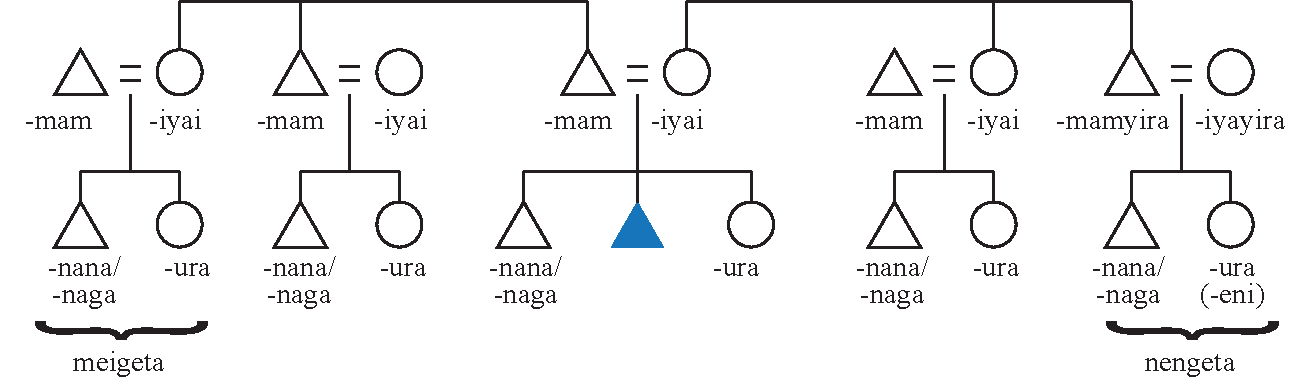
\includegraphics[width=\textwidth]{figures/Holton_ch5_fig8.pdf}
\caption{Kiraman terminology in ego's and ascending generation (male ego)}
\label{fig:5:8}
\end{figure}  


\begin{table}[p]
\centering
\caption{Kiraman\ilt{Kiraman} kinship\ist{kinship} terms}
\label{table_kiraman_terms}
\begin{tabular}{lL{4.5cm}L{5cm}}
\mytopline
\textit{-mam} & F, FB, FZH, MZH & father, paternal uncle\\
\textit{{}-iyai} & M, MZ, FZ, FBW & mother, aunt\\
\textit{{}-ma(m)yira} & MB & maternal uncle\\
\textit{{}-iyayira} & MBW & maternal uncle's wife\\
\textit{{}-nana} & meB, feZ, FeB & same-sex elder sibling, \\
& elder paternal uncle \\
\textit{{}-naga} & myB, fyZ, FyB & same-sex younger sibling, \\
& younger paternal uncle \\
\textit{{}-ura} & mZ, fB & opposite-sex sibling\\
\textit{baki} & eB, eZ & elder sibling\\
\textit{ika} & yB, yZ & younger sibling\\
\textit{nengeta} & MB lineage & maternal uncle's lineage\\
\textit{meigeta} & FZ lineage & paternal aunt's lineage\\
\textit{yiramei} & mMBD & man's female maternal cross-cousin\\
\textit{yiranen} & fFZS & woman's male paternal cross-cousin\\
\textit{{}-edat} & WF, HF, DH, WM, HM, SW & parent-in-law, child-in-law\\
\textit{gei nen} & H & husband\\
\textit{gei mei} & W & wife\\
\textit{{}-eni} & mMBD, fFZS, (mFZS), (fMBD), mZH, WB & marriageable cross-cousin, (sibling's marriageable cross-cousin), man's brother-in-law\\
\textit{{}-amo} & fBW, HZ, mZH, WB & in-law, affine of ego's generation\\
\textit{{}-ina} & HeBW, WeZH & elder same-sex in-law\\
\textit{{}-mol} & HW & husband's (other) wife\\
\textit{{}-iyol} & C & classificatory child\\
\textit{{}-amoku} & HWC & child of husband's (other) wife\\
\mybottomline
\end{tabular}
\end{table}

Kiraman ascending terminology distinguishes ego's mother's brother's side through the terms \textit{-ma(m)yira} MB and \textit{-iyayira} MBW, transparently derived from the terms \textit{-mam} `father' and \textit{-iyai} `mother' plus \textit{yira} `base'. Other ascending relationships referring to ego's parent's siblings and their spouses are denoted using the terms for mother and father modified by \textit{baki} `older' or \textit{ika} `younger', depending on the age of the referent relative to ego's mother or father, respectively. In particular, father's sister is not distinguished from mother except through the use of a relative age modifier. Descendants of one's \textit{-mayira} and \textit{-iyayira} can be optionally denoted \textit{nengeta}. The reciprocal term is \textit{meigeta}. Neither \textit{nengeta} nor \textit{meigeta} is used as a term of address. Descending terminology does not distinguish between biological children and children of ego's siblings but rather groups C, BC, ZC together as \textit{-iyol} `classificatory child'.

As in Blagar\il{Blagar}, affines in ascending and descending generations are referred to by a single term \textit{-edat}. The term \textit{-edat} is its own reciprocal. Affines in ego's generation are referred to as \textit{-amo}. A man's brother-in-law may optionally be denoted \textit{-eni}, the same term which is used to denote marriageable cross-cousins. Spouses of same-sex siblings may refer to each other as siblings, following the relative ages of their spouses. In addition, a more respectful term for the elder of two spouses of same-sex siblings is \textit{-ina.} Thus, if A and B are brothers, and A is older than B, then B's wife calls A's wife \textit{neina}, while A's wife calls B's wife \textit{ika} `younger sibling'. 

 



Terms which are not gender-specific may be optionally specified for gender using the terms \textit{mei} `female' and \textit{nen} `male'. For example, \textit{-iyol mei} `daughter' and \textit{{}-edat nen} `father-in-law'. Kiraman\il{Kiraman} also has a distinct term \textit{-mol} by which one wife refers to another in a polygamous marriage. These women refer to each other's children as \textit{-amoku}. 


\subsection{Adang}\label{sect_adang}
The Adang\il{Adang} kinship\is{kinship} system also lacks an obligatory terminological distinction between siblings and (parallel and cross) cousins. There are two primary sets of terminologies for classificatory siblings. The first distinguishes older and younger siblings, \textit{matu} and \textit{di'}, respectively. The second includes the single term \textit{-uding} `sibling'. None of these terms is specified for gender, but each may be optionally modified with \textit{ob} `female' or \textit{lote} `male' when one wishes to specify gender. Thus, \textit{no'uding lote} `my female sibling', i.e., `my sister'. 

\begin{figure}[h]
 %\includegraphics[width=6.2583in,height=1.9165in,width=\textwidth]{fc7457c206664b669ab0bf2a407db9b7-img9}
 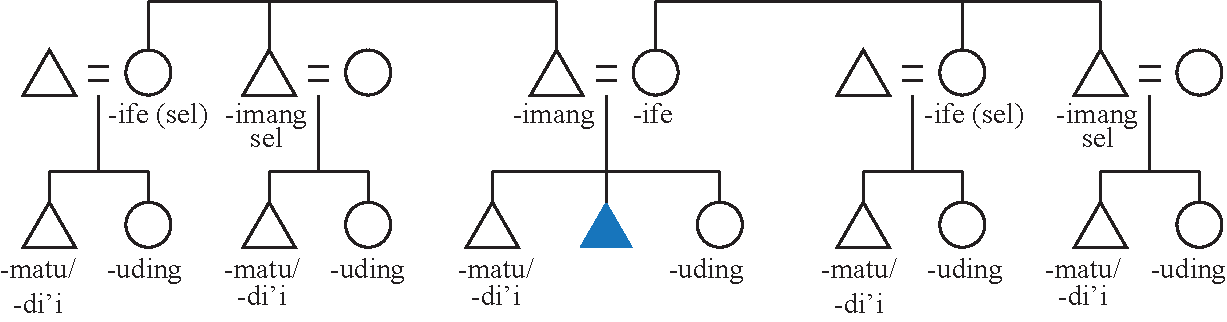
\includegraphics[width=\textwidth]{figures/Holton_ch5_fig9.pdf}
\caption{Adang terminology in ego's and ascending generation (male ego)}
\label{fig:5:9}
\end{figure}  

The age-based \textit{matu}/\textit{{}-di'} terminology has a connotation of intimacy and is preferred for biological siblings, though \textit{-uding} can be used in this context as well. The children of one's father's brother and one's mother's sister (i.e., parallel cousins) are generally referred to as \textit{-uding}, though the \textit{matu}/\textit{{}-di'} terminology is also acceptable here in certain contexts. The children of one's father's sister and one's mother's brother (i.e., cross-cousins) are almost always referred to as \textit{-uding}; the \textit{matu}/\textit{{}-di'} terminology seems to be unacceptable here. This yields a kind of covert cross-cousin category, as shown in Table \ref{tab:5:5}. 




\begin{table}
\centering

\caption[Adang sibling terminologies]{Adang\ilt{Adang} sibling terminologies   \mbox{({\checkmark}=preferred, ?=acceptable,  x=unacceptable)}}
\label{tab:5:5}

\begin{tabular}{rcc}

\mytopline
& \textit{-matu/-di'} & \textit{-uding} \\
\midrule
biological siblings (B, Z)  &  {\checkmark} & ?\\
parallel cousins (MZC, FBC) &      ?        & {\checkmark}\\
cross-cousins (MBC, FZC)    &      x        & {\checkmark}\\
\mybottomline
\end{tabular}
 

\end{table}  

However, there is wide leeway in the application of this sibling terminology, and the choice between the two sibling terminologies depends greatly on pragmatics.\enlargethispage{1em}

Co-existing with the two sibling terminologies described above is an additional layer of sibling terminology which does explicitly distinguish cross-cousins. The terms are \textit{ob ai} `man's female cross-cousin' (mMBD, mFZD) and \textit{lote ai} `woman's male cross-cousin' (fMBS, fFZS). These terms are reciprocal, so that if A refers to B as \textit{no'ob ai}, then B refers to A \textit{nolote ai}. The terms derive from the gender terms \textit{ob} `female' and \textit{lote} `male' plus \textit{ai} `child', but when possessed the gender terms are identical to the terms for spouses, thus these cross-cousin terms translate literally as `husband child' and `wife child'. Though not used as terms of address, the \textit{ob ai}/\textit{lote ai} relationship is very salient to speakers, even though the referents may continue to refer to each other using the regular sibling terminology. These terms refer strictly to opposite-sex cross-cousins; Adang\il{Adang} has no special terminology for same-sex cross-cousins. 

A fourth optional distinction in ego's generation is made using the term \textit{asel}, derived from \textit{sel}, a term sometimes translated as `tree' (Malay `pohon') but which actually refers to `area underneath, base', as in \textit{ti sel } `area beneath the tree' (see {\SS} \ref{sec:5:3}). The term \textit{asel} denotes one's mother's brother and descendants. Thus, maternal cross-cousins of either gender are \textit{asel}. Like \textit{ob ai}/\textit{lote ai}, the term \textit{asel} is not used as a term of address but rather as a description, delineating those descendants of my mother's (brother's) family. The entire mother's brother's lineage can be referred to as \textit{asel em}, derived from \textit{em} `old'. 

The term \textit{sel} also occurs in ascending terminology \textit{-imang sel} `uncle' (MB, FB) and \textit{-ife sel} `aunt' (MZ, FZ). My consultants struggled with the latter term, maintaining that \textit{sel} has no role in \textit{nife sel} and that the modifier could equally be omitted. In contrast, \textit{-imang sel} is clearly distinguished from \textit{-imang} `father'\textit{.} It appears that the use of the modifier \textit{sel} has been extended by analogy.


 


\begin{table}\centering 
\begin{tabular}{p{3cm}L{3cm}L{5cm}}
\mytopline
\textit{{}-imang} & F & father\\
\textit{{}-ife} & M, MZ, FZ & mother, aunt\\
\textit{{}-imang sel} & FB, MB & uncle\\
\textit{{}-ife sel} & FZ, MZ & aunt\\
\textit{{}-matu} & eB, eZ, FeBC, FeZC, MeBC, MeZC & elder classificatory sibling\\
\textit{{}-di'} & yB, yZ, FyBC, FyZC, MyBC, MyZC & younger classificatory sibling\\
\textit{{}-uding} & B, Z, FBC, FZC, MBC, MZC & sibling\\
\textit{{}-'ob ai} & mMBD, mFZD & man's opposite-sex cross-cousin\\
\textit{{}-lote ai} & fMBS, fFZS & woman's opposite-sex cross-cousin\\
\textit{asel} & MB, MBC & mother's brother and descendants\\
\textit{asel em} & MB lineage & mother's brother's lineage\\
\textit{{}-'ob} & W & wife\\
\textit{{}-lote} & H & husband\\
\textit{{}-afeng} & WB, W & affine of ego's generation\\
\textit{bap} & 2nd ascending generation & grandparent\\
\textit{bap turtur} & 3rd or more ascending generation & ancestors\\
\textit{{}-'ai} & C, BC, ZC & classificatory child\\
\textit{di'ing} & CC & classificatory grandchild\\
\mybottomline
\end{tabular}

\caption{Adang\ilt{Adang} kinship\ist{kinship} terms}
\label{table_adang_terms}
\end{table}
A woman's family may be additionally distinguished via the use of a second genitive pronominal\is{pronoun} prefix paradigm. In addition to the usual possessive\is{possession} paradigm with the back \textit{o} vowel grade, Adang\il{Adang} distinguishes a second paradigm referred to as ``contrastive'' \citep{Haan2001} which employs a front vowel grade. A male ego may use the contrastive paradigm to refer to the children of his wife's siblings, e.g., \textit{ne'ai} `my wife's sibling's child' (WZC, WBC). This term is only used by men; there is no corresponding term by which women can distinguish their husband's sibling's children. The terms with contrastive prefix are not used as vocatives. The usual term for referring to one's biological children as well as those of one's siblings and one's spouse's siblings is \textit{no'ai} `my child', with optional specification for gender, \textit{no'ai ob} `my daughter' and \textit{no'ai lote} `my son'.

Affines in ego's generation are denoted by the term \textit{{}-afeng}, a term which essentially means `other' (cf. Abui \textit{afenga}). Included in this category are the spouses of one's siblings, as well as one's spouse's siblings and their spouses. No special terms for affines in ascending and descending generations have been documented. Instead, ascending and descending affines are referred to by the same parent and child terminology used for consanguinal (biological) relations. 

The second ascending generation above ego is denoted \textit{bap} `grandparent', while more distant ascending generations are denoted \textit{bap turtur} `ancestors'. One's  child or one's sibling is denoted \textit{'ai}, while the second descending generation below ego is denoted by \textit{di'ing} `grandchild'. These terms can be further specified for gender with \textit{ob} `female' or \textit{lote} `male'. 

 
\subsection{Abui}\label{sect_abui}\ilt{Abui}
Abui\il{Abui} resembles Adang\il{Adang} in having two primary terminologies for ego's generation, neither of which distinguishes between biological siblings and (parallel or cross) cousins. The first set of terminology is age-based and distinguishes \textit{-naana} `older sibling/cousin' from \textit{-kokda} (or \textit{-nahaa}) `younger sibling/cousin'.\footnote{\citet[56]{Nicolspeyer1940} lists \textit{nahaa} rather than \textit{kokda} as the term for `younger sibling', while both terms appear in \citet{KratochvilEtAl2008kamus}. My consultants prefer the latter term.}  Gender is not distinguished. A second terminology is gender-based and distinguishes \textit{-moknehi} `same-sex sibling/cousin' from \textit{-ura} `opposite-sex sibling/cousin'. The choice between the two terminologies is pragmatically based and has nothing to do with the distinction between siblings and cousins. The gender-based terminology is more appropriate for older ages, whereas the age-based terminology is more appropriate for young children. The same-sex term \textit{-moknehi} can also be used with broader semantics as a term of address even for those who are not immediate kin (Figure \ref{fig:5:10}).

\begin{figure}[h]
 %\includegraphics[width=6.2583in,height=2.3244in,width=\textwidth]{fc7457c206664b669ab0bf2a407db9b7-img10}
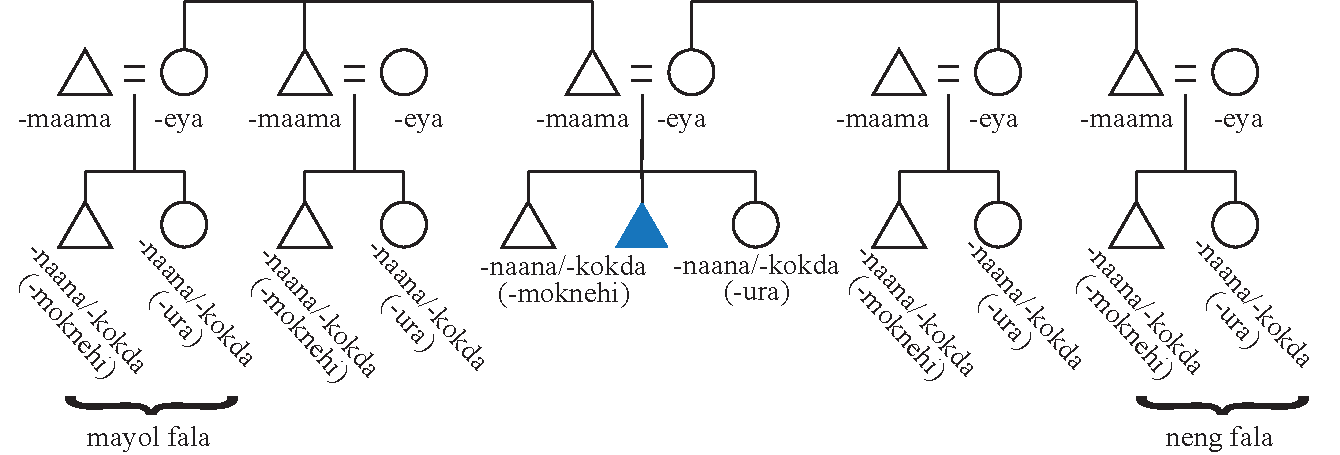
\includegraphics[width=\textwidth]{figures/Holton_ch5_fig10.pdf}
\caption{Abui terminology in ego's and ascending generation (male ego)}
\label{fig:5:10}
\end{figure}  

An additional layer of terminology for ego's generation distinguishes cross-cousins via the terms \textit{neng fala} `mother's brother's child' and \textit{mayol fala} `father's sister's child'. These terms can be used as vocatives without a possessive prefix, or they may be possessed\is{possession} to describe the relationship, e.g., \textit{neneng fala} `my mother's brother's child'. In this sense they contrast with Adang \textit{ob ai/lote ai}, which cannot be used as vocatives. The terms \textit{neng fala} and \textit{mayol fala} are also reciprocals of each other, so that ego's \textit{neng fala} calls ego \textit{mayol fala}. These terms are derived from the words for `man' and `woman', plus \textit{fala} `house'. Descendants of one's \textit{neng fala} are referred to as \textit{kalieta fala}, literally `elder house', while descendants of one's \textit{mayol fala} are referred to as \textit{wiil fala}, literally `child house'.\footnote{The Takalelang variety of Abui described here differs from the Atimelang variety described by \citet{Nicolspeyer1940}. Rather than the terms \textit{wiil fala} and \textit{kalieta fala}, in Atimelang one finds \textit{kokda fala} and \textit{feng fala}, respectively. These terms are semantically similar: \textit{wiil} `child' vs. \textit{kokda} `younger'; and \textit{kalieta} `old' vs. \textit{feng} `elder'. However, Nicolspeyer indicates that the Atimelang terms \textit{kokda fala} and \textit{feng fala} are used to refer to the descendants of one's parents' younger and elder siblings, respectively (1940: 46).}  

The relationship between descendants of opposite-sex siblings is diagrammed in Figure \ref{fig:5:11}. The referents labeled A and B are children of opposite-sex siblings, that is, cross-cousins. A calls B \textit{mayol fala}, literally `female house', while B calls A \textit{neng fala}, literally `male house'. The children of A refer to the children of B as \textit{wiil fala}, literally `child house', while the children of B refer to the children of A as \textit{kalieta fala}, literally `elder house'. 

\begin{figure}[h]
\centering
 %\includegraphics[width=3.2917in,height=2.0555in,width=\textwidth]{fc7457c206664b669ab0bf2a407db9b7-img11}
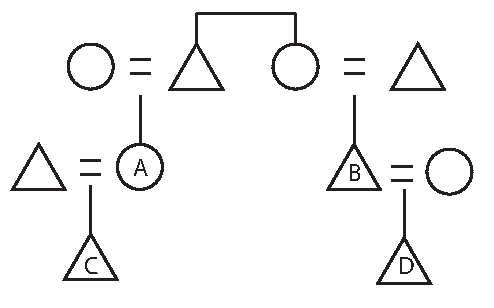
\includegraphics[width=6.5cm]{figures/Holton_ch5_fig11.pdf}
\caption[Abui descendants of opposite-sex siblings]{Abui\ilt{Abui} descendants of opposite-sex siblings. C refers to D as wiil fala `child house'; D refers to C as \textit{kalieta fala} `elder house'}
\label{fig:5:11}
\end{figure}  

These terms do not depend on the gender of the referent but rather on the genders of the respective siblings from which they descend. C belongs to the male side and is thus the elder house; D belongs to the female side and is thus the younger house. These terms can be used across generations as well, so that A may refer to D as either \textit{wiil fala} or \textit{mayol fala}; and D may refer to A as either \textit{kalieta fala} or \textit{neng fala}.

These descending generation terms reveal the asymmetry in the Abui\il{Abui} system. The mother's side, through the mother's brother, is viewed as elder, while the father's side, through the father's sister, is viewed as a child. This distinction is further reflected throughout various ceremonial obligations. \textit{Mayol fala} must always respect \textit{neng fala}, while \textit{neng fala} cares for \textit{mayol fala} in an endearing way. Ascending terms in Abui distinguish siblings of one's biological parents via the modifiers \textit{fing} `elder, eldest' and \textit{kokda} `younger'. There is no distinction between opposite-sex and same-sex siblings of one's parents.

Affine terms in Abui\il{Abui} depend on the relative gender of the referent. Opposite-sex affines are \textit{-biena}. Male affines are \textit{-raata}. Female affines are \textit{-mooi}. These terms remain the same for ego's generation as well as for ascending and descending generations. Thus, \textit{-raata} denotes a man's wife's brother and the reciprocal, a man's sister's husband; and \textit{-raata} also denotes a man's wife's father and the reciprocal, a man's daughter's husband. The opposite-sex affine term \textit{-biena} can also be used by spouses of opposite-sex siblings to refer to each other. 

A distinct term \textit{-mool} is used by women to refer to their husband's other wives. This term may also be used by women who are married to brothers, likely reflecting traditional levirate marriage. Further evidence of this practice can be found in the traditional Abui\il{Abui} adage, \textit{moknehi haba amool ri} `sisters become \textit{amool}', said when two sisters either marry two brothers or marry a single husband. 

Abui\il{Abui} shares with Kamang\il{Kamang} ({\SS} \ref{sec:5:2}.7) an elaborate distinction in generational levels, distinguishing three descending and four ascending generations, as shown in Table \ref{table_abui_terms}.

\begin{table}
\small
\begin{tabular}{lL{4cm}L{4cm}}
\mytopline
\textit{{}-maama} & F, FB, MB & father, uncle\\
\textit{{}-eya} & M, MZ, FZ & mother, aunt\\
\textit{{}-maama fing} & MeB, FeB, MeZH, FeZH & elder uncle\\
\textit{{}-maama kokda} & MyB, FyB, MyZH, FyZH & younger uncle\\
\textit{{}-eya fing} & MeZ, FeZ, MeBW, FeBW & elder aunt\\
\textit{{}-eya kokda} & MyZ, FyZ, MyBW, FyBW & younger aunt\\
\textit{{}-naana} & eB, eZ & elder sibling\\
\textit{{}-kokda (-nahaa)} & yB, yZ & younger sibling\\
\textit{{}-ura} & mZ, fB & opposite-sex sibling\\
\textit{{}-moknehi} & mB, fZ & same-sex sibling\\
\textit{{}-neng fala} & MB, MBC & maternal uncle and descendants\\
\textit{{}-mayol fala} & FZ, FZC & paternal aunt and descendants\\
\textit{{}-kalieta fala} & descendants of \textit{neng fala} & maternal uncle's lineage\\
\textit{{}-wiil fala} & descendants of \textit{mayol fala} & paternal aunt's lineage\\
\textit{{}-mayol} & W & wife\\
\textit{{}-neng} & H & husband\\
\textit{{}-mool} & HW, HBW & husband's (other) wife\\
\textit{{}-mooi} & HZ, fBW & woman's sister-in-law\\
\textit{{}-biena} & HB, WZ, mBW, fZH & woman's brother-in-law, man's sister-in-law\\
\textit{{}-raata} & WM, WF, WB, DH, mZH & man's brother-in-law, man's parent-in-law,\par man's son-in-law\\
\textit{{}-moku} & C & child\\
\textit{{}-ratala} & CC & grandchild\\
\textit{{}-rak beeka} & CCC & great-grandchild\\
\textit{{}-kuta} & 2nd ascending generation & grandparent\\
\textit{{}-tungtung} & 3rd ascending generation & great-grandparent\\
\textit{{}-taita} & 4th ascending generation and above & great-great-grandparent\\
\mybottomline
\end{tabular}

\caption{Abui\ilt{Abui} kinship\ist{kinship} terms}
\label{table_abui_terms}
\end{table}
\newpage

\subsection{Kamang}\label{sect_kamang}\ilt{Kamang}
Kamang\il{Kamang} kinship\is{kinship} is described by \citet{Stokhof1977} based on the Ateita dialect. The system described here is based on variants spoken in Apui and neighboring Silaipui districts, drawing on field work in 2010 and 2013. The two descriptions generally agree, though Stokhof is often more restrictive in delineating the semantics of certain terms. For example, Stokhof restricts the gender-based terms for ego's generation (\textit{-namuk} `same-sex sibling/cousin' and \textit{-naut} `opposite-sex sibling/cousin') to those linked through the ego's father's side. My consultants report no such restriction. This broader interpretation is also found in \citet{SchapperEtAl2011kamus}, where \textit{-namuk} is defined as ``same sex cousin, FBS/FZS for male or FBD/FZD for female''. It may well be that the Kamang\il{Kamang} system has bleached somewhat in the four decades since Stokhof's research was conducted, so that terms which were once restricted to father's side have broadened to include both mother's and father's side.

A slightly different example type of discrepancy can be found in the terms \textit{-namuk ela} and \textit{-naut ela}, which both \citet{Stokhof1977} and   \citet{SchapperEtAl2011kamus} define as cross-cousins on the mother's side. There is some disagreement about these terms among my consultants. Some speakers reject the terms altogether preferring instead to use the cross-cousin term \textit{lammi}. Others accept the terms but acknowledge that the unmodified versions \textit{-namuk} and \textit{-naut} can also be used in this context. Most likely there are two overlapping terminological systems at work here: one distinguishing cross-cousins via the \textit{lammi}/\textit{malemi} terminology; and the other distinguishing the mother's side via \textit{ela}. Nonetheless, Kamang\il{Kamang} today as described here still maintains significant skewing toward the maternal side in the first ascending generation. 

Kamang\il{Kamang} has two primary sets of terminology for ego's generation. The first is age-based, distinguishing \textit{-naka} `elder sibling/cousin' and \textit{-kak} `younger sibling/cousin'. These terms are synonymous with \textit{-idama} and \textit{-idika}, respectively, and these latter terms are more commonly used in their vocative form, \textit{dama} and \textit{dika}, respectively. A second set of terminology is gender-based and distinguishes \textit{-namuk} `same-sex sibling/cousin' from \textit{-naut} `opposite-sex sibling/cousin'. The same-sex term \textit{-namuk} is less likely to be used to indicate biological siblings, in which case the age-based terms are preferred. The term \textit{-namuk} can be used more generally as a friendly way of greeting persons of the same gender as ego, even if not closely related. For both sets of terminology a biological sibling (or at least closer) relationship can be indicated by compounding the terms with \textit{kang}. Thus, \textit{nenaut kang} `my (male speaking) sister' (See Figure \ref{fig:5:12}). 


\begin{figure}[h]
%\includegraphics[width=6.2583in,height=1.9165in,width=\textwidth]{fc7457c206664b669ab0bf2a407db9b7-img12}
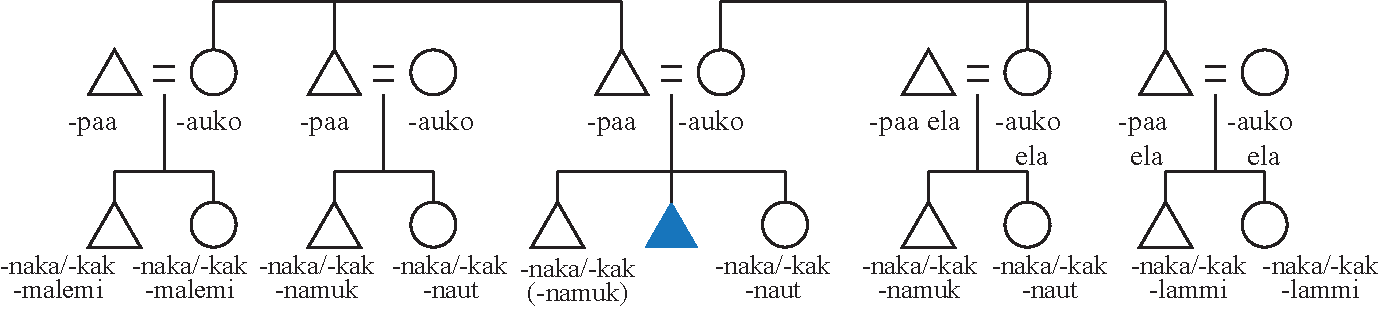
\includegraphics[width=\textwidth]{figures/Holton_ch5_fig12.pdf}
\caption{Kamang\ilt{Kamang} terminology in ego's and ascending generation (male ego) }
\label{fig:5:12}
\end{figure}  

 

While Stokhof reports the use of the gender-based terms for cross-cousins as well as parallel cousins, my consultants prefer to limit the use of these terms to parallel cousins (and siblings). A different set of terminology is used for cross-cousins, distinguishing \textit{lammi} `maternal cross-cousin' (MBC) and \textit{malemi} `paternal cross-cousin' (FZC). These terms are not distinguished for gender, the gender of either ego or referent, but they are reciprocal, so that if A calls B \textit{lammi}, then B calls A \textit{malemi.} In contrast to other Alor-Pantar languages, there is a strong taboo against marriage between cross-cousins (see {\SS} \ref{sec:5:4}). The cross-cousin terms are not used as terms of address except in very specific formal contexts; instead, the usual age-based sibling terms are used. The \textit{lammi-malemi} relationship is inherited through generations, so that the children of \textit{lammi} and \textit{malemi} also refer to each other as \textit{lammi} and \textit{malemi}. However, the restriction on marriage between \textit{lammi} and \textit{malemi} expires after three generations.

Kamang\il{Kamang} terminology in the first ascending generation is unique among the languages described in this chapter. Paternal terms are merged with father and mother, but maternal terms are distinguished via the modifier \textit{ela}. This is shown in Figure \ref{fig_kamang_ascending}. Some speakers merge both the maternal and paternal sides in casual reference, though they still optionally distinguish the maternal side via \textit{ela}. In vocative address, all members of the first ascending generation are addressed as \textit{nepaa} `my father' or \textit{nauko} `my mother'.

\begin{figure}[b]
 %\includegraphics[width=6in,height=1.8083in,width=\textwidth]{fc7457c206664b669ab0bf2a407db9b7-img13}
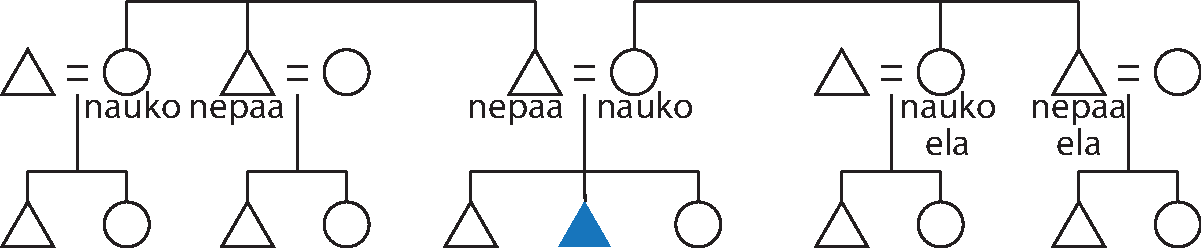
\includegraphics[width=\textwidth]{figures/Holton_ch5_fig13.pdf}
\caption{Kamang\ilt{Kamang} terms in first ascending generation}
\label{fig_kamang_ascending}
\end{figure}  
 

 \begin{table}[p]
\centering
\small

\begin{tabular}{p{3cm}L{3cm}p{5cm}}
\mytopline
\textit{{}-paa} & F, FB, FZH & father, paternal uncle\\
\textit{{}-auko} & M, FZ, FBW & mother, paternal aunt\\
\textit{{}-paa idama} & FeB, (MeB) & elder (paternal) uncle\\
\textit{{}-paa idika} & FyB, (MyB) & younger (paternal) uncle\\
\textit{{}-auko idama} & FeZ, (MeZ) & elder (paternal) aunt\\
\textit{{}-auko idika} & FyZ, (MyZ) & younger (paternal) aunt\\
\textit{{}-paa ela} & MB, MZH & maternal uncle\\
\textit{{}-auko ela} & MZ, MBW & maternal aunt\\
\textit{{}-naka} & eB, eZ, MeBC, FeBC, MeZC, FeZC & elder classificatory sibling\\
\textit{{}-kak} & yB, yZ, MyBC, FyBC, MyZC, FyZC & younger classificatory sibling\\
\textit{{}-namuk} & (mB), (fZ), fFBD, mFBS, fMZD, mMZS & same-sex classificatory sibling\\
\textit{{}-naut} & mZ, fB, fFBS, mFBD, fMZS, mMZD & opposite-sex classificatory sibling\\
\textit{lammi} & MBC & maternal cross-cousin\\
\textit{malemi} & FZC & paternal cross-cousin\\
\textit{dum} & C, MBC, MZC, FBC, FZC & classificatory child\\
\textit{lam} & H & husband\\
\textit{male} & W & wife\\
\textit{{}-nabeng} & affine of ego's generation & \\
\textit{{}-noy} & HZ, fBW & woman's sister-in-law\\
\textit{{}-mot} & HBW, WZH, HW & \\
\textit{{}-nataka} & WF, HF, WM, HM, DH, SW & parent-in-law, child-in-law\\
\textit{{}-ben} & SWF, SWM, DHF, DHM & child-in-law's parent\\
\textit{tale dum} & WC, HC & step-child\\
\textit{tale namuk} & MC, FC & step-sibling\\
\mybottomline
\end{tabular}
\normalsize
\caption[Kamang kinship terms]{Kamang\ilt{Kamang} kinship\ist{kinship} terms.{\footnotemark} }
\label{table_kamang_terms}
\end{table}


Affines in ego's generation are denoted by \textit{-nabeng}. This term is its own reciprocal. Female affines may be optionally called \textit{-noy} by a female ego. Spouses of same-sex siblings refer to each other as \textit{-mot}. This same term is used by wives to refer to other wives sharing the same husband. In the ascending and descending generations only a single affine term is used, namely, \textit{-nataka}. This term is independent of gender and is its own reciprocal. 
 

\footnotetext{The Kamang\ilt{Kamang} terms \textit{lamta} and \textit{maleta} have been omitted from this list. \citet{Stokhof1977} equates \textit{lamta} and \textit{dum lam} but does not list \textit{maleta}. Stokhof's definition of both \textit{dum lam}  and \textit{dum male} is much broader, applying to a large group of kin in ego's generation. I was unable to confirm this definition with my consultants.}



\subsection{Wersing}\ilt{Wersing}\label{sect_wersing}
Wersing does not make an obligatory distinction between siblings and cousins, though cross-cousins are covertly distinguished, as discussed below. There are two sets of terminology for classificatory siblings (hereafter simply siblings), age-based and gender-based. The age-based terminology distinguishes \textit{-nang} `older sibling' from \textit{-kaku} `younger sibling'. The gender-based terminology consists of the single term \textit{-arudi} `opposite-sex sibling'. Thus, only the age-based terms may be used for same-sex siblings. The age-based terms are most commonly used also for opposite-sex siblings; the gender-based term is considered more formal or endearing.

In addition to the classificatory sibling terminologies, same-sex children of opposite-sex siblings, i.e., same-sex cross-cousins, are referred to as \textit{-beng}. This same term is used for affines in ego's generation which are related through opposite-sex siblings. Thus, \textit{-beng} denotes mZH, WB, fBW, HZ. These are precisely the people whose children can call ego's children \textit{-beng}. A man's female maternal cross-cousin (mMBD) is not referred to or addressed as \textit{-beng} but is instead tacitly considered to be a spouse, at least until the man marries someone else. Instead, a man's female maternal cross-cousin may be referred to (but not addressed) as \textit{-mei deng}, literally `female female-side'. A woman in turn refers to her male paternal cross-cousin by the reciprocal term \textit{-limi deng}, literally, `male female-side'.\footnote{My fieldnotes are actually inconclusive as to whether \textit{-mei deng} and \textit{-limi deng} can be applied also to a man's female paternal cross-cousin (mFZD) and the reciprocal woman's male maternal cross-cousin (fMBS). However, I suspect that they cannot, in which case these terms are then skewed toward the man's mother's brother's side in a way similar to that found in Kiraman (see {\SS} \ref{sec:5:4}.2).}  The term \textit{deng} itself derives from a plural marker but in this context denotes a man's mother's brother's family.

Affines in ascending and descending generations are referred to by the term \textit{-tat} `spouse's parent, child's spouse'. In contrast to languages like Teiwa\il{Teiwa}, Wersing\il{Wersing} lacks distinct terms for MB and FZ which may be employed for affines in the ascending generation. Hence, the term \textit{-tat} is used reciprocally. The spouse of one's opposite sex sibling is \textit{{}-beng} and thus treated as a same-sex cross-cousin. The same term denotes the reciprocal relationship of one's spouse's opposite-sex sibling. The spouse of one's spouse's opposite-sex sibling thus counts as an opposite-sex cross-cousin and is thus ``marriageable''. However, this person is generally referred to with an age-based sibling term \textit{{}-nang} or \textit{{}-kaku}, though never as \textit{{}-arudi}, as that term is reserved for consanguine relations. 

In the first ascending generation ego's parent's siblings and their spouses are all referred to by one of the terms \textit{-paidem} `older uncle', \textit{-par} `younger uncle', \textit{-yidem} `older aunt', \textit{-yar} `younger aunt' (see Figure \ref{fig14_wersing}). The terms \textit{-pa} `father' and \textit{-ya} `mother' are reserved for biological and adoptive parents only. No distinction is made between maternal and paternal aunts and uncles. The elder terms are clearly derived from \textit{-pa} `father' and \textit{-ya} `mother' plus \textit{idem} `eldest'; however, speakers do not recognize a morphological division here; nor do they view these terms as referring literally to an older or younger father or mother. The reciprocal term for \textit{{}-paidem}, \textit{{}-par}, \textit{{}-yidem}, and \textit{{}-yar}, as well as \textit{-pa} and \textit{{}-ya}, is simply \textit{{}-ol} `child'. 

\begin{figure}[h]
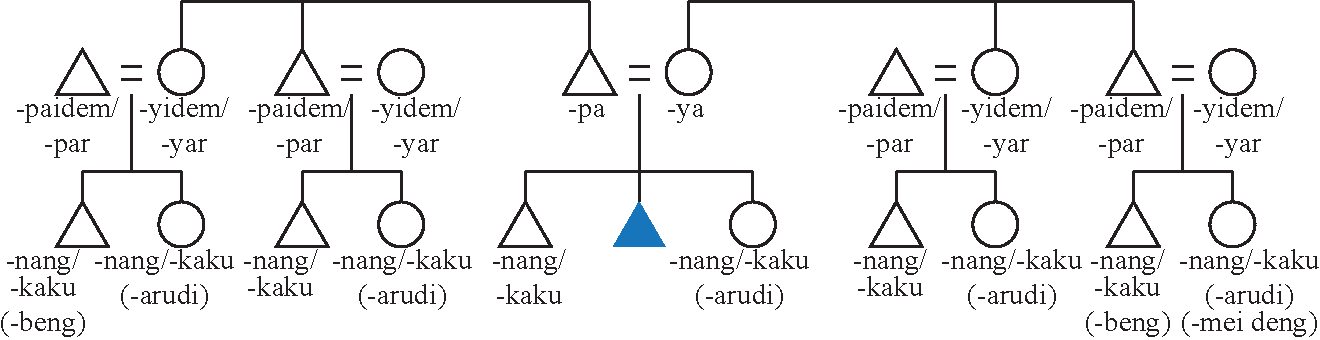
\includegraphics[width=\textwidth]{figures/Holton_ch5_fig14.pdf}
\caption{Wersing\ilt{Wersing} terminology in ego's and ascending generation (male ego)}
\label{fig14_wersing}
\end{figure}
 

The term \textit{-tam} is used for kin in the second ascending and descending generations. Thus, grandchildren and grandparents address each other by the same term, \textit{netam}. For ascending generations above this the term \textit{\mbox{-}nakar}, literally `earlier times', is used. For descending generations below this the term \textit{{}-silu}, literally `sprout, bud', is used. 
 

\begin{table} 
\centering

\begin{tabular}{lL{4.5cm}p{5cm}}
\mytopline
\textit{{}-pa} & F & father\\
\textit{{}-ya} & M & mother\\
\textit{{}-paidem} & FeB,MeB & elder uncle\\
\textit{{}-par} & FyB, MyB & younger uncle\\
\textit{{}-yidem} & FeZ, MeZ & elder aunt\\
\textit{{}-yar} & FyZ, MyZ & younger aunt\\
\textit{{}-nang} & eB, eZ & elder sibling\\
\textit{{}-kaku} & yB, yZ & younger sibling\\
\textit{{}-arudi} & mZ, fB & opposite-sex sibling\\
\textit{{}-tat} & CH, CW, WM, WF, HM, HF & parent in-law, child in-law\\
\textit{{}-beng} & fMBD, fFZD, mMBS, mFZS, mZH, WB, fBW, HZ & parallel cousin\\
\textit{{}-limi deng} & fFZS, (fMBS ?) & woman's male paternal (and maternal?) cross-cousin\\
\textit{{}-mei deng} & mMBD, (mFZD ?) & man's female maternal (and \par paternal?) cross-cousin\\
\textit{{}-ol} & C, BC, ZC & classificatory child\\
\textit{{}-tam} & 2nd ascending/descending generation & grandchild, grandparent\\
\textit{{}-nakar} & 3rd ascending generation and above & great-grandchild,\par great-grandparent\\
\textit{{}-silu} & 3rd descending generation and below & great-great-grandchild, \par
great-great-grandparent\\
\mybottomline
\end{tabular}
\caption{Wersing\ilt{Wersing} kinship\ist{kinship} terms}
\label{table_wersing_terms}
\end{table}

\newpage
\section{Summary and comparison of kinship terms}\ist{kinship}\label{sec:5:3}
Given the close genealogical relationships between the Alor-Pantar languages, there is relatively little shared kinship vocabulary. \citet{HoltonRobinsonTVposition} reconstruct just three kinship terms: `father', `child', and `older sibling', though it should be noted that the methodology used to elicit vocabulary for that study may have overlooked potential cognate forms with differing semantic values. To these three we might add `mother', for which it is difficult to propose an actual reconstruction, since it appears to be composed of a sequence of two vowels, and the vowel correspondences have yet to be worked out (see Table \ref{tab:5:10}). Note that Kamang\il{Kamang} \textit{-auko} `mother' likely contains a fossilized endearment suffix \textit{-ko}. Also, while reflexes of `older sibling' are not found in the three Pantar languages in this sample, the reconstruction is supported by Nedebang\il{Nedebang} \textit{-nang}. Two additional forms `younger sibling' and `opposite-sex sibling' may also be reconstructable (see Table \ref{tab:5:14}), but those forms are not as widely attested as these four.

 

\begin{table}[h]
\centering

\begin{tabular}{lllll} & `mother' & \parbox{1.5cm}{`father'\\ *-mam} &\parbox{1cm}{`child'\\*-uaqal} & \parbox{3cm}{`older sibling'\\{}-*nan(a)}\\
\mytopline
Western Pantar\il{Western Pantar} & \textit{{}-au} & \textit{{}-iba} & \textit{{}-wakal} & \textit{(-ikkar)}\\
Teiwa\ilt{Teiwa} & \textit{(-xala')} & \textit{{}-oma'} & \textit{{}-oqai} & \textit{(-ka'au)}\\
Blagar\ilt{Blagar} & \textit{{}-iva} & \textit{{}-imang} & \textit{{}-oqal} & \textit{(-ku)}\\
Kiraman\ilt{Kiraman} & \textit{{}-iyai} & \textit{{}-mam} & \textit{{}-ol} & \textit{{}-nana}\\
Adang\ilt{Adang} & \textit{{}-ife} & \textit{{}-imang} & \textit{{}-'ai} & \textit{(-matu)}\\
Abui\ilt{Abui} & \textit{{}-eya} & \textit{{}-maama} & \textit{(-moku)} & \textit{{}-naana}\\
Kamang\ilt{Kamang} & \textit{{}-auko} & \textit{{}-paa} & \textit{(dum)} & \textit{{}-naka}\\
Wersing\ilt{Wersing} & \textit{{}-ya} & \textit{{}-pa} & \textit{{}-ol} & \textit{{}-nang}\\
\mybottomline
\end{tabular}
\caption{Cognate kinship vocabulary, with reconstructed pAP\ilt{proto-Alor-Pantar} forms where available (non-cognate forms in parentheses)}
\label{cognate_vocab}
\label{tab:5:10}
\end{table}

Unfortunately, the reconstructions in Table \ref{cognate_vocab} do not shed light on the actual structure of the kinship\is{kinship} system, and the tag glosses given for the reconstructions should be taken as a rough indication of the relevant kin category. For example, reflexes of *mam `father' may refer to `F' alone, `F, FB', or even `F, FB, MB'. In order to understand the nature of the original Alor-Pantar kinship system we must compare the semantic structure of the kin terms, particularly as they relate to the distinction of cross-cousins and mother's brother.

The semantic distribution of the terms corresponding to the six kin type primitives in the first ascending generation are given in Table \ref{table_kinship_categories}. The table shading indicates kin type primitives which are classed together with the same term. The table reveals that even where kinship\is{kinship} vocabulary is cognate across languages, the terms may have differing semantic values. For example, Kamang\il{Kamang} \textit{-paa} and Wersing\il{Wersing} \textit{-pa} `father' are obviously cognate, but the meaning of the Kamang\il{Kamang} form is also extended to `father's brother' but not to `mother's brother', which has a distinct term in Kamang\il{Kamang}. In contrast, Wersing\il{Wersing} use the same term \textit{-paidem/-par}.

 

\begin{table}[h]
\centering 

\begin{tabular}{rcccccc} 	
\mytopline
		& F~ 			& FB 			& MB 			& M~ 		& MZ 	& FZ\\ 
\hhline{~------}
Western Pantar\ilt{Western Pantar} 	& {\darkgreycell} 	& {\darkgreycell} 	&  			& {\blackcell} 	& {\blackcell} 	& {\lightgreycell}	\\
 \hhline{~------}
        \\
 \hhline{~------}
Teiwa\ilt{Teiwa} 		& {\darkgreycell} 	& {\darkgreycell} 	&  			&  {\blackcell}	& {\blackcell} 	& {\lightgreycell}	\\
\hhline{~------}
        \\
\hhline{~------}
Blagar\ilt{Blagar} 		& {\darkgreycell} 	& {\darkgreycell} 	&  			& {\blackcell} 	& {\blackcell} 	& {\lightgreycell}	\\
\hhline{~------}
        \\
\hhline{~------}
Kiraman\ilt{Kiraman} 	& {\darkgreycell} 	& {\darkgreycell} 	&  			& {\blackcell} 	& {\blackcell} 	& {\blackcell}	\\
\hhline{~------}
        \\
\hhline{~------}
Adang\ilt{Adang} 		& {\darkgreycell} 	&  			& \vline\,\vline\,\vline\,\vline\,\vline\,\vline\,\vline\,\vline\,\vline\,\vline\,\vline 	& {\blackcell} 	& {\blackcell} 	& {\blackcell}	\\
\hhline{~------}
        \\
\hhline{~------}
Abui\ilt{Abui} 		& {\darkgreycell} 	& {\darkgreycell} 	&  {\darkgreycell}	& {\blackcell} 	& {\blackcell} 	& {\blackcell}	\\
 \hhline{~------}
        \\
\hhline{~------}
Kamang\ilt{Kamang} 		& {\darkgreycell} 	& {\darkgreycell} 	&  			& {\blackcell} 	&  {\lightgreycell}		& {\blackcell}	\\
\hhline{~------}\\
\hhline{~------}
Wersing\ilt{Wersing} 	& {\darkgreycell} 	&  			&  			& {\blackcell} 	&  {\lightgreycell}		& {\lightgreycell}	\\ 
\hhline{~------}
\mybottomline
\end{tabular}

\caption{Comparison of kinship\ist{kinship} categories in the first ascending generation. Shading indicates kin type primitives which are classed together with the same term.}
\label{table_kinship_categories}
\label{tab:5:11}
\end{table}

For the purposes of this comparison optional age-based modifier terms are excluded. Thus, while Abui\il{Abui} may refer to MB as \textit{-maama fing} or \textit{-maama kokda}, according to whether alter is older or younger, respectively, than ego's parent, this term is here considered to be classed with \textit{-maama} F. Wersing\il{Wersing} presents some difficulties for this convention, since the Wersing\il{Wersing} terms for parents' siblings are derived from the terms for M and F together with suffixes \textit{idem} and \textit{{}-r}, depending on whether alter is older or younger, respectively, than ego's parent. However, in contrast to the Abui\il{Abui} situation, these suffixes are not semantically transparent to Wersing\il{Wersing} speakers. While Abui\il{Abui} \textit{-maama kokda} is transparently `younger father', Wersing\il{Wersing} \textit{-par} `FyB, MyB' is not seen by Wersing speakers as related in any way to \textit{-pa} `father'. Hence, for the purposes of this analysis the opaque Wersing\il{Wersing} suffixes are retained. Were the suffixes to be discarded the Wersing\il{Wersing} system would look like that found in Abui, which has only two primary terms in the ascending generation, corresponding to males and females.

Most of the languages described here have a distinct term for MB. The one marginal case is found in Adang\il{Adang}, which classes MB and FB together as \textit{imang sel}. However, only MB and his descendants can be denoted by the term \textit{asel}. This suggests that the \textit{sel} modifier has been extended from MB to FB. In any case, MB is still distinguished by a distinct term. That leaves only Abui\il{Abui} and Wersing lacking a distinct MB term. 

For the female ascending terms, there is less consensus across the languages. The Pantar languages all distinguish FZ from M and MZ, but three languages class all female kin of the first ascending generation together. Kamang\il{Kamang} follows yet another pattern which distinguishes both male and female kin on the mother's side.

Comparing terminology across the six languages which have a distinct MB term reveals that the MB term in most cases has been derived from the term for father plus a modifier which can be translated as `base' (Table \ref{distinct_MB}). The presence of the `base' formative is most transparent in Blagar\il{Blagar}, Kiraman\il{Kiraman}, and Kamang\il{Kamang}, where the forms \textit{era}, \textit{yira}, and \textit{ela}, respectively, can be identified. In Western Pantar\il{Western Pantar} and Teiwa\il{Teiwa} the rhotic is likely a reduced form of the `base' formative, though it does not occur synchronically as such. In the Western Pantar\il{Western Pantar} case a comparison with the Lamma dialect, where the word for `father' is \textit{-iba}, shows that the rhotic is unique to the MB term. The Adang\il{Adang} formative \textit{sel} also means `base' but is used to denote MB without the \textit{-mang} term.

 


\begin{table}[p]
\centering
\begin{tabular}{l>{\it}l>{\it}l}
\mytopline
& \rm F & \rm MB\\
\midrule  
Western Pantar\ilt{Western Pantar} (Lamma) & {}-iba & {}-irasi\\
Teiwa\ilt{Teiwa} & {}-oma' & {}-umeer\\
Blagar\ilt{Blagar} & {}-imang & {}-imang era\\
Adang\ilt{Adang} & {}-mang & asel\\
Kiraman\ilt{Kiraman} & {}-mam & {}-mamyira\\
Kamang\ilt{Kamang} & {}-paa & {}-paa ela\\
\mybottomline
\end{tabular}
\caption{Comparison of F and MB terms in those languages which have a distinct MB term}
\label{distinct_MB}
\label{tab:5:12}
\end{table}

The broad semantics of the `base' forms are well articulated for Blagar\il{Blagar} in \citet[156]{Steinhauer1993}. Cognates and semantically similar terms are found across many of the Alor Pantar languages (Table \ref{table_botanic}). A prototypical usage would be Kamang\il{Kamang} \textit{bong ela} `base of tree'. This usage of the `base' modifier derives from a more widespread botanic metaphor which is common throughout Eastern Indonesia \citep{Fox1995}. Among the eight languages considered here only Wersing\il{Wersing} appears to completely lack a kinship\is{kinship} modifier based on a botanic term (Table \ref{tab:5:13}).
  
\begin{table}[p]

\begin{tabular}{rlp{1cm}L{5cm}}
\mytopline
language & modifier & gloss & kinship usage\\
\midrule  
Western Pantar\ilt{Western Pantar} & \textit{haila} & `base' & close relative\\[.3em]
Teiwa\ilt{Teiwa} & \textit{yis} & `fruit' & \textit{-bruman yis} `marriageable cross-cousin'\\[.3em]
Blagar\ilt{Blagar} & \textit{era} & `base' & \textit{{}-imang era} MB, \textit{{}-iva era} FZ\\[.3em]
\multirow{2}{*}{Kiraman\ilt{Kiraman}} & \textit{geta}  & `base'
& \textit{meigeta} FZC, \textit{nengeta} MBC\\
 &\textit{yira}& `tree' & \textit{{}-iyai yira} MBW, \textit{{}-mam yira} MB\\[.3em]
Adang\ilt{Adang} & \textit{sel} & `base' & \textit{{}-imang sel} MB, FB; \textit{asel} MBC\\[.3em]
Abui\ilt{Abui} & \textit{iya} & `trunk' & \textit{pi iya nuku} `we are from one tree; related'\\[.3em]
Kamang\ilt{Kamang} & \textit{ela} & `base' & \textit{{}-paa ela} MB, \textit{{}-auko ela} MZ\\[.3em]
Wersing\ilt{Wersing} & {}-{}- & {}-{}- & {}-{}-\\
\mybottomline
\end{tabular}

\caption{Use of botanic metaphors in Alor-Pantar kinship\ist{kinship} terms }
\label{table_botanic}
\label{tab:5:13}
\end{table}

Turning now to ego's generation we find that these kinship\is{kinship} terms often come in multiple overlapping sets of terminologies, and choice between terminologies may be pragmatically governed. Age-based systems for siblings are found in all of the languages except Blagar\il{Blagar}. Gender-based systems for siblings are found in all languages except Adang\il{Adang}. Most of the gender-based systems distinguish between same-sex and opposite-sex siblings. Teiwa\il{Teiwa} is unique in having gender-based sibling terms which are absolute and not dependent on relative genders of ego and alter. None of the sibling terms can be reconstructed at the level of proto-Alor-Pantar\il{proto-Alor-Pantar} with much confidence. Only `younger sibling' and `opposite-sex sibling' have a very wide distribution across the languages, as shown in Table \ref{table_siblings}. But even these forms do not obey established consonant correspondences, so they are likely to have diffused.

 

\begin{table}[h]
\centering

\begin{tabular}{rcc}
\mytopline
& \parbox{3cm}{{}-*kak \\ `younger sibling'} & \parbox{4cm}{*-ura\\ `opposite-sex sibling'}\\
\midrule
Western Pantar\ilt{Western Pantar} & \textit{{}-iaku} & \textit{{}-{}-}\\
Teiwa\ilt{Teiwa} & \textit{(-bif)} & \textit{{}-{}-}\\
Blagar\ilt{Blagar} & \textit{{}-{}-} & \textit{{}-edi}\\
Kiraman\ilt{Kiraman} & \textit{{}-naga} & \textit{{}-ura}\\
Adang\ilt{Adang} & \textit{(-di)} & \textit{{}-{}-}\\
Abui\ilt{Abui} & \textit{{}-kokda} & \textit{{}-ura}\\
Kamang\ilt{Kamang} & \textit{{}-kak} & \textit{{}-naut}\\
Wersing\ilt{Wersing} & \textit{{}-kaku} & \textit{{}-arudi}\\
\mybottomline
\end{tabular}

\caption{Tentative reconstruction of sibling terms }
\label{table_siblings}
\label{tab:5:14}
\end{table} 

The choice between age-based and gender-based systems is for the most part pragmatically governed, with the latter being more formal or distant. In some languages there is a strong preference for use of the age-based terms for same-sex siblings and the gender-based terms for opposite-sex siblings. In Western Pantar\il{Western Pantar} this preference is strictly manifested so that age-based terms are used only for same-sex siblings, while distinct terms are used for opposite-sex siblings. In addition, Western Pantar\il{Western Pantar} has distinct terms for male speaking and female speaking for `elder (same-sex) sibling' and `opposite-sex sibling'. 

  All of the languages have terminology for distinguishing cross-cousins. However, the languages vary as to whether: (i) cross-cousins are obligatorily distinguished; (ii) when cross-cousins are distinguished, marriageable (opposite-sex) are obligatorily distinguished from non-marriageable (same-sex) cross-cousins; (iii) when cross-cousins are distinguished, those on MB side are distinguished from those on FZ side; and (iv) there are cross-cousin terms distinct from terms referring to the entire lineage. These distinctions are summarized in Table \ref{table_cross-cousin_distinctions}.

 

\begin{table}[h]
\centering

\begin{tabular}{r|c|c|c|c|}
\mytopline
\multicolumn{1}{c}{}& 
\multicolumn{1}{c}{\parbox{2cm}{\centering~\\obligatory}} & 
\multicolumn{1}{c}{\parbox{2cm}{\centering marriageable\\distinguished}}  & 
\multicolumn{1}{c}{\parbox{2cm}{\centering maternal \\ distinguished}}  & 
\multicolumn{1}{c}{\parbox{2cm}{\centering distinguished \\from lineage}} 
\\
\hhline{~----}
W Pantar & {\darkgreycell} & {\darkgreycell} &  & {\darkgreycell}\\
\hhline{~----}
Teiwa  & {\darkgreycell} &  &  & {\darkgreycell}\\
\hhline{~----}
Blagar & {\darkgreycell} &  &  & {\darkgreycell}\\
\hhline{~----}
Kiraman&  &  & {\darkgreycell} & {\darkgreycell}\\
\hhline{~----}
Adang  &  & {\darkgreycell} & {\darkgreycell}  & \\
\hhline{~----}
Abui   &  &  & {\darkgreycell} & \\
\hhline{~----}
Kamang &  &  & {\darkgreycell} & \\
\hhline{~----}
Wersing&  & {\darkgreycell} &  & {\darkgreycell}\\
\hhline{~----}
\mybottomline
\end{tabular}
\vspace{1cm}
\caption{Comparison of cross-cousin distinctions} 
\label{table_cross-cousin_distinctions}
\label{tab:5:15}
\end{table}

The languages fall into two groups along the first parameter above. Only the three Pantar languages Western Pantar\il{Western Pantar}, Teiwa\il{Teiwa}, and Blagar\il{Blagar} obligatorily distinguish cross-cousins from siblings. In these languages cross-cousins form a distinct category and are not considered siblings. In the other languages cross-cousins can be distinguished when necessary, but they can also be referred to using the sibling terminology. Only Western Pantar\il{Western Pantar} obligatorily distinguishes same-sex from opposite-sex cross-cousins. In Teiwa\il{Teiwa} and Blagar\il{Blagar} a single term applies to cross-cousins regardless of gender, while those of opposite gender may be optionally distinguished. As can be seen from Table \ref{tab:5:16}, it is not possible to reconstruct any of the cross-cousin terminology for these languages. The Teiwa\il{Teiwa} term \textit{-ian} may be related to the term \textit{-ianqai} `brother'. No inferences can be drawn regarding the historical origin of the cross-cousin terms in Western Pantar\il{Western Pantar} and Blagar\il{Blagar}. 

 


\begin{table}[h]
\centering

\begin{tabular}{llll} 
\mytopline
& general & same-sex & opposite-sex\\
\midrule
Western Pantar\ilt{Western Pantar} &  & \textit{{}-'ar / -ingtamme} & \textit{{}-baddang}\\
Teiwa\ilt{Teiwa} & \textit{{}-ian} &  & \textit{{}-dias}\\
Blagar\ilt{Blagar} & \textit{{}-ebheang} &  & \textit{{}-boromung}\\
\mybottomline
\end{tabular}

\caption{Comparison of cross-cousin terms}
\label{table_cross-cousin_terms}
\label{tab:5:16}
\end{table}

Only in Western Pantar can the opposite-sex cross-cousin term be used as a form of address. In Teiwa and Blagar this term is avoided in address by using the general form. In Wersing the opposite-sex cross-cousin term has a strong association with marriage and is thus avoided in address by using the sibling terminology instead. 

  The remaining five languages, all spoken on Alor, classify siblings and (parallel and cross) cousins together. However, these languages may optionally distinguish cross-cousins, and in doing so also distinguish between maternal and paternal cross-cousins. In Kiraman\il{Kiraman}, Abui\il{Abui}, Kamang\il{Kamang}, and Wersing\il{Wersing} maternal cross-cousins are referred to with a term derived from the word for `male', while paternal cross-cousins are referred to with a term derived from the word for `female'. In Adang\il{Adang} only maternal cross-cousins are distinguished; there is no separate term for paternal cross-cousins. Terms for maternal and paternal cross-cousins are compared in Table \ref{table_maternal-paternal_cross-cousins}. Kiraman\il{Kiraman} also has a term \textit{-ueni} which refers specifically to a man's maternal opposite-sex cross-cousin (mMBD) and reciprocally to a woman's paternal opposite-sex cross-cousin (fFZS). This term then extends to a man's paternal same-sex cross-cousin (mFZS), since this person is a potential spouse of one's \textit{-eni} and is thus also referred to as \textit{-eni.} 
 


\begin{table}[h]
\centering
\begin{tabular}{llll}
\mytopline
& MBC & FZC & derivation\\
\midrule  
Kiraman\ilt{Kiraman} & \textit{nengeta} & \textit{meigeta} & \textit{geta} `trunk'\\
Adang\ilt{Adang} & \textit{asel} & \textit{{}-{}-} & \textit{sel} `base'\\
Abui & \textit{neng fala} & \textit{mayol fala} & \textit{fala} `house'\\
Kamang\ilt{Kamang} & \textit{lammi} & \textit{malemi} & \textit{mi} `located'\\
Wersing\ilt{Wersing} & \textit{limideng} & \textit{meideng} & \textit{deng} `side'\\
\mybottomline
\end{tabular}

\caption{Maternal and paternal cross-cousin terms}
\label{table_maternal-paternal_cross-cousins}
\label{tab:5:17}
\end{table}

Here again the terms for maternal and paternal cross-cousins do not admit a reconstruction. Though Kiraman\il{Kiraman}, Adang\il{Adang}, Kamang\il{Kamang}, and Wersing\il{Wersing} derive the cross-cousin terms from the words for `male' and `female', they do so by the addition of different (and non-cognate) formatives. 

 Affine terminology also exhibits significant variation across the languages. Where distinct terminology for cross-cousins and mother's brother exists, this same terminology is applied to affines. In ego's generation this follows logically from the observation that the spouse of ego's sibling should ideally be that sibling's cross-cousin, hence also cross-cousin to ego. Similar reasoning suggests that the parent of ego's spouse should be called by the same term as ego's mother's brother or father's sister, since those persons would be the parent of ego's cross-cousin, who would be ego's ideal marriage partner. However, only Western Pantar and Teiwa actually adopt this strategy for spouse's parent and affines of ego's generation. The terminology for affines is summarized in Table \ref{table_affines}. The forms listed for spouse's sibling apply also to the reciprocal sibling's spouse, with appropriate adjustment for reference. Thus, Kamang\il{Kamang} \textit{-noy} is both `woman's brother's wife' (fBW) and also `husband's sister' (HZ).

\begin{table}[h]
\centering

\begin{tabular}{p{2cm}>{\it}p{3.75cm}>{\it}l>{\it}r} 
\mytopline
& spouse's sibling  & spouse's parent & child's spouse\\
\midrule  

Western Pantar\ilt{Western Pantar} 
 
& -baddang {\rm (mBW, fZH)}\newline -ingtamme {\rm (fBW)}\newline -'ar {\rm (mZH)} & -irasi & -airas\\[3pt]

Teiwa\ilt{Teiwa} & -ian {\rm (mZH, fBW)} \newline -dias {\rm (mBW, fZH)} & -umeer/-xaler & -rat\\[3pt]

Blagar\ilt{Blagar} & -des & \multicolumn{2}{c}{\textit{-idat}}\\[3pt]

Kiraman\ilt{Kiraman} & -amo \newline -eni & \multicolumn{2}{c}{\textit{-dat}}\\[3pt]

Adang\ilt{Adang} & -afeng &  & \\[3pt]

Abui\ilt{Abui} & -biena {\rm (mBW, fZH)} \newline -amooi {\rm (fBW)} \newline -raata {\rm (mZH)} & -biena & -raata\\[3pt]

Kamang\ilt{Kamang} & -nabeng \newline -noy {\rm (fBW)} & \multicolumn{2}{c}{\textit{-nataka}}\\[3pt]

Wersing\ilt{Wersing} & -beng {\rm (fBW, mZH)} & \multicolumn{2}{c}{\textit{-tat}}\\[3pt]


\mybottomline
\end{tabular}

\caption{Comparison of affine terms}
\label{table_affines}
\label{tab:5:18}
\end{table}

A single affine term *\textit{dat} can be tentatively reconstructed at the level of proto-Alor Pantar\il{proto-Alor-Pantar}. This term probably had the general meaning of `affine kin' but was then restricted to affines in the descending generation as affines in the ascending generation were replaced by terms denoting the parents of cross-cousins. Crucially, the reconstructed affine term is distinct from terms denoted cross-cousins, suggesting that the original kinship\is{kinship} terminology was not based on a direct exchange system where affines would be cross-cousins.

\section{Marriage prescriptions}\label{sec:5:4}
As discussed in the previous section, special terminology for cross-cousins is found in most of the Alor-Pantar languages. However, the role of cross-cousins and that of mother's brother varies significantly across the languages. In some languages the terminology denotes a privileged marriageable relationship, based on symmetrical exchange. In other languages there is asymmetrical exchange with the mother's brother's side serving as the wife-givers. In yet other languages there is no marriage prescription, even though cross-cousins may be terminologically distinguished and  play important roles in exchange relationships. 

Some common threads in marriage practices are found in all of the Alor-Pantar languages. Descent is patrilineal and almost always patrilocal, and exchange between descent groups plays a central role in social structure, linking lineages beyond the time span of the actual marriage. The bronze kettledrum, or \textit{moko}, plays a central symbolic role in the exchange of bride wealth, and the relative valuations of the kettledrums serves to regulate the direction of circulation of women. Distinguishing between the ideology of marriage and the actual practice of marriage is difficult without a more detailed ethnographic study of marriage and exchange, and such a study is unfortunately beyond the scope of this chapter, which is necessarily preliminary.\footnote{There is as of yet still no detailed ethnographic description of marriage practices in Alor, though the reader may consult \citet{Nicolspeyer1940} on Abui\il{Abui}; \citet{Stokhof1977} on Kamang\il{Kamang}; and \citet{Steinhauer2010} on Blagar\il{Blagar}. Additional information on marriage practices can be gleaned from the ethnographic introductions to reference grammars of Teiwa\il{Teiwa} \citep{Klamer2010grammar}, Abui\il{Abui} \citep{Kratochvil2007}, and Klon\il{Klon} \citep{Baird2008}. \citet{Forman1980} describes marriage customs in Makasae\il{Makasae}, a related language spoken in East Timor.} With that in mind this section focuses on a description of marriage prescriptions in the Alor-Pantar languages. 

\begin{figure}[h]
\centering
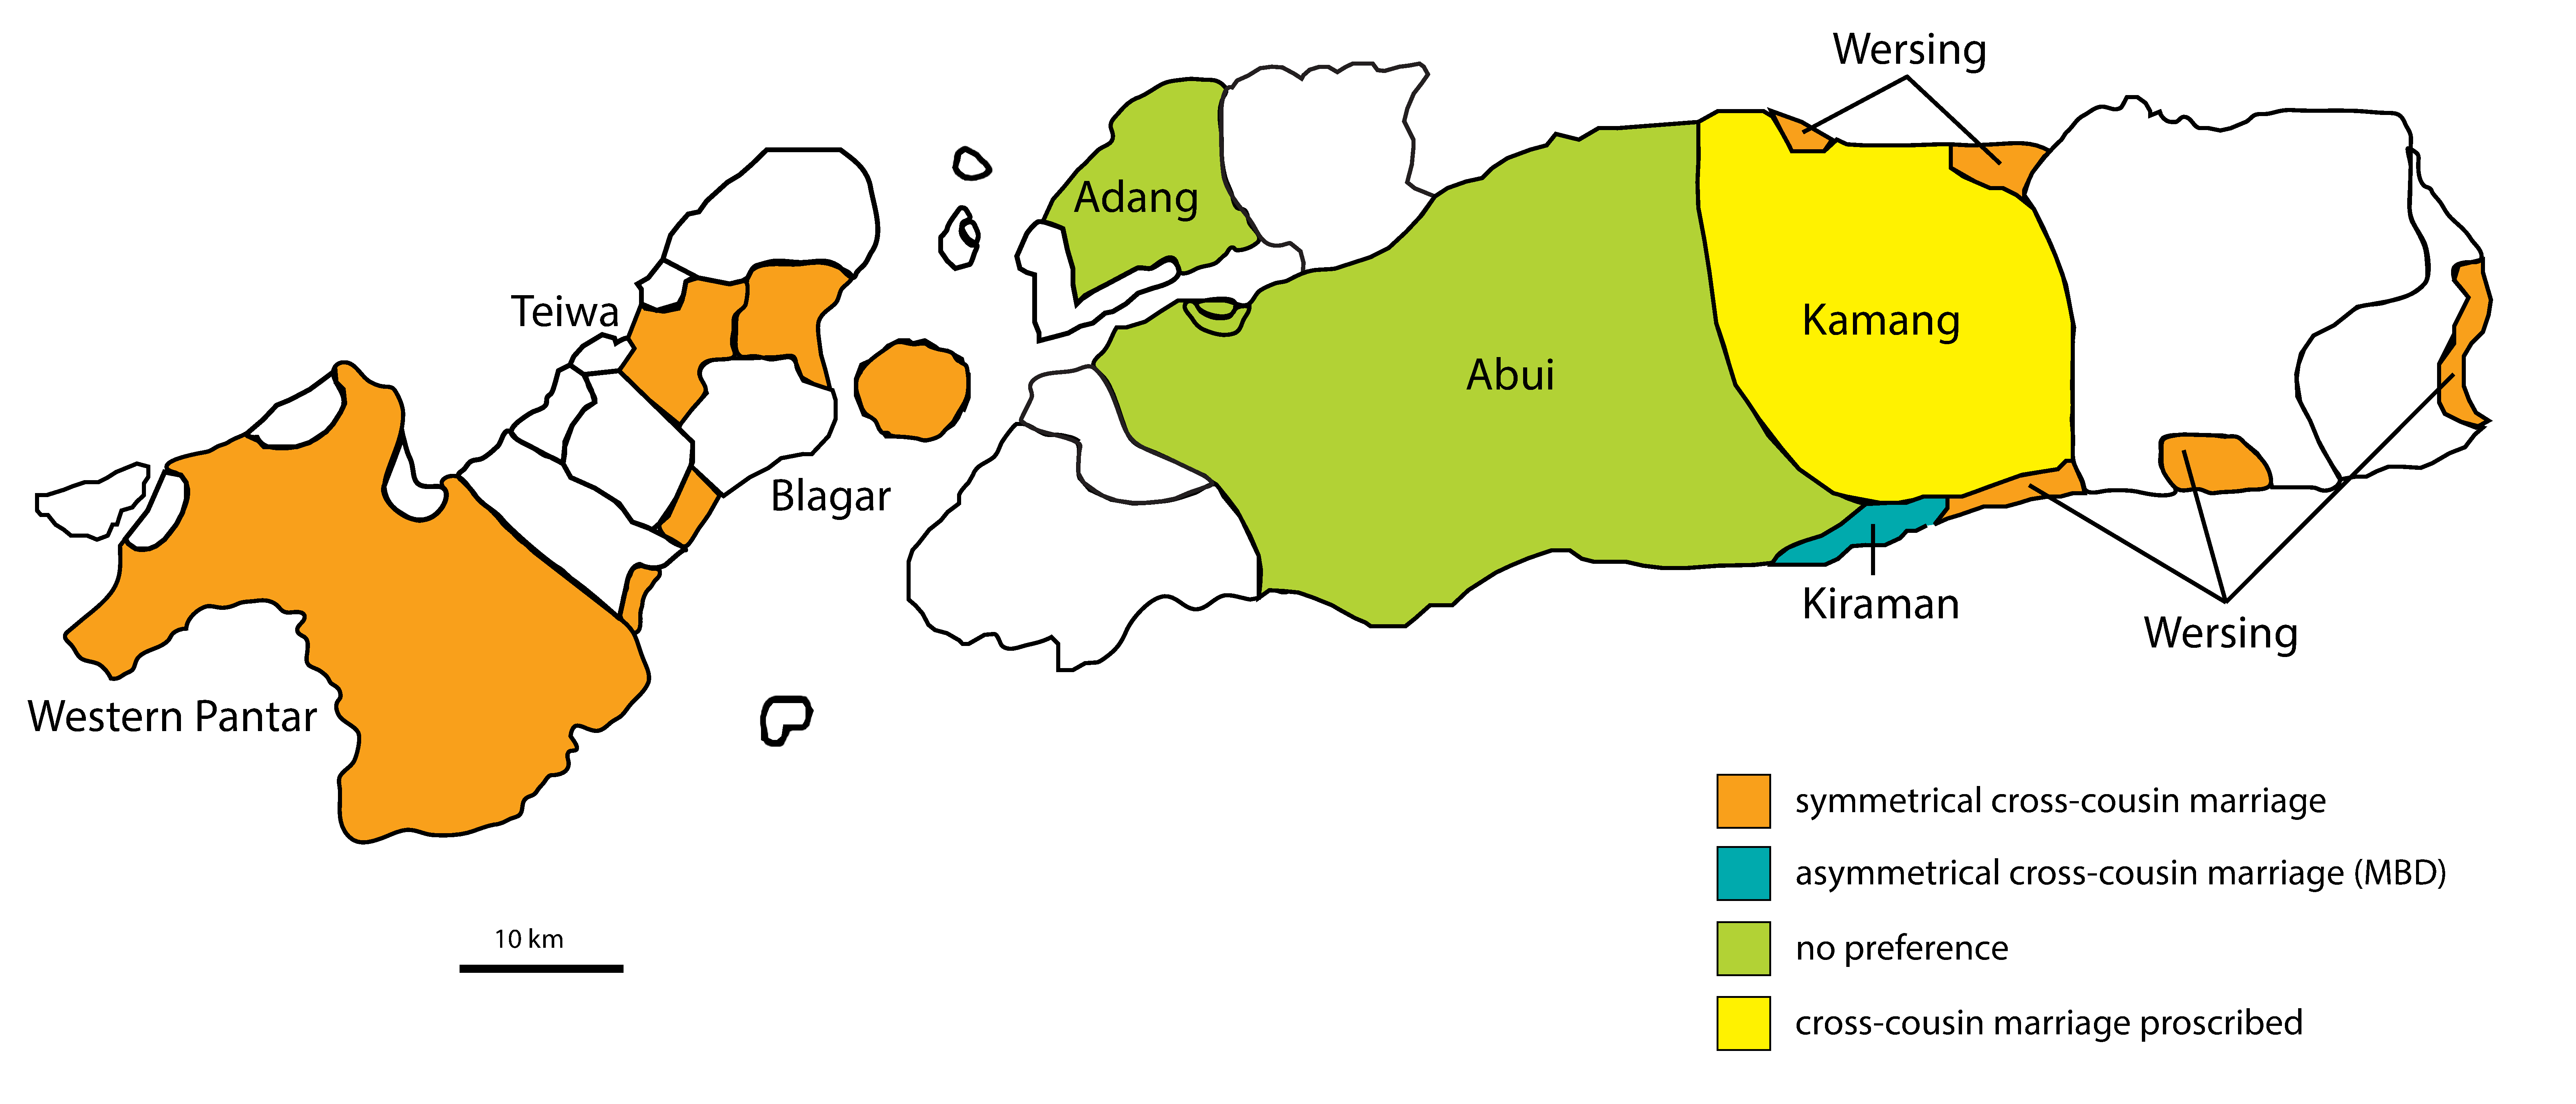
\includegraphics[width=\textwidth]{figures/Holton_ch5_fig16.pdf}
\caption{Geographic distribution of languages according to type of marriage prescription}
\label{fig:5:16}
\end{figure}

Three broad patterns of marriage prescription can be identified, as follows (see Figure~\ref{fig:5:16}): 
\begin{enumerate}
\item[(i)] symmetrical systems in which the man draws a wife from either the mother's brother's or the father's sister's lineage; 
\item[(ii)] asymmetrical systems in which the mother's brother's lineage serves as wife-giver; 
\item[(iii)] non-prescriptive systems with no preference for marriage outside certain specific proscriptions;
\end{enumerate}

In the following subsections I discuss each of these systems in turn. Within the third category we can further distinguish systems in which cross-cousin marriage is explicit	ly proscribed. As shown in Figure \ref{fig:5:16} systems of marriage prescription are regionally distributed. Symmetrical systems are found throughout Pantar and on the eastern coast of Alor. Asymmetrical systems are found only in Kiraman\il{Kiraman}, also located on the eastern coast of Alor. Non-prescriptive systems, including the completely proscriptive system in Kamang\il{Kamang}, are found in Central Alor and the Bird's Head. The marriage prescriptions do not match exactly with kinship\is{kinship} terminology, proving the point that  terminology does not determine practice. Exchange has a number of dimensions in Alor-Pantar which will only be illuminated with further study.

\subsection{Symmetrical exchange}
In Western Pantar\il{Western Pantar}, Teiwa\il{Teiwa}, Blagar\il{Blagar}, and Wersing\il{Wersing} cross-cousin marriage is held up as the ideal. There is symmetrical exchange with no skewing toward either the mother's or the father's side. That is, there is no preference for marriage to ego's mother's brother's child over ego's father's sister's child. Systems of symmetrical exchange are found at the two extremes of the archipelago: among the languages of Pantar in the west and in Wersing along the eastern coast of Alor (Figure \ref{fig:5:16}). Here I focus on Western Pantar\il{Western Pantar}, since I am most familiar with the marriage customs there. I have no data on the actual extent of cross-cousin marriage, though I suspect it is quite rare. In Kedang\il{Kedang}, an Austronesian language\il{Austronesian language(s)} spoken immediately to the west of Western Pantar\il{Western Pantar}, \citet[88]{Barnes1980} found a conformance rate of 58\% with the cross-cousin marriage prescription rule. I suspect that the rate in Western Pantar\il{Western Pantar} is similar, though it was likely much greater in the past.\footnote{\citet{Steinhauer2010} suggests that among the Blagar\ilt{Blagar} of Pura strict adherence to cross-cousin marriage had broken down by the time of the Japanese occupation in the 1940s.} Western Pantar\il{Western Pantar} treats all marriages as if they were between cross-cousins. However, Western Pantar recognizes a distinction between marriage established through classificatory cross-cousins, and marriage to persons outside the region who cannot be traced as cross-cousins. The former are \textit{-baddang haila}, literally `base cross-cousin'; while the latter are \textit{-baddang wang gamining}, literally `cross-cousin included'. The \textit{-baddang wang gamining} very literally included in that, once married, they are treated as if they were in fact \textit{-baddang} for the purposes of identifying further kinship relationships via transitivity. There is a certain circularity to this system in that \textit{-baddang} defines the ideal marriageable relationship, yet any marriage is treated \textit{as if} the partners were \textit{-baddang}, effectively establishing the \textit{-baddang} relationship by fiat. 

Very rarely marriage may occur between more distantly related siblings, that is, between a man and his \textit{-aipang wang gamining} or between a woman and her \textit{-aiyang wang gamining}. This could happen for instance with an affine relative of one's sibling when that sibling marries into another clan. The participants in such a marriage may refer to each other as \textit{wallang} (i.e., \textit{-baddang}), since that is considered the ideal marriage relationship. However, this relationship is referred to as \textit{burang nattang}, literally `getting together shaking hands'. At one time such a practice resulted in much stronger reprobation. In contrast, marriage between a man and his \textit{-aipang haila} or between a woman and her \textit{-aiyang haila} is never permitted, even today.

As in Western Pantar, in Blagar all marriages are effectively treated as if they were cross-cousin marriages. As noted in {\S} \ref{sect_blagar}, if marriage between ego and his or her cross-cousin is actually realized, then ego's \textit{-imang era} and \textit{-iva era} become simply \textit{-idat} `in-laws'. Similarly, these new parents-in-law now also refer to ego as \textit{-idat} rather than \textit{-bhilang}. The spouse of ego continues to be referred to by these parents-in-law as a classificatory child \textit{-oqai}, since ego's cross-cousin is the child of ego's \textit{-imang era} and \textit{-iva era} (now \textit{-idat}). Significantly, this remains the case even when \textit{-bhilang} does not marry their cross-cousin. That is, whomever ego's \textit{-bhilang} marries becomes ego's classificatory child, regardless of whether they held this status prior to the marriage. This relationship may then be propagated recursively. The result is that ego's spouse is always treated as the child of ego's potential parents-in-law (MB or FZ), hence ego's cross-cousin.

\subsection{Asymmetrical exchange}\label{sect_asymmetrical_exchange}
\label{bkm:Ref247334472}Kiraman\il{Kiraman} practices matrilineal cross-cousin marriage, in which the ideal marriage relationship is between a man and his matrilineal cross-cousin, i.e., his mother's brother's daughter, whom he denotes with the term \textit{-eni}. This system is asymmetrical in that marriage between a man and his patrilineal cross-cousin is prohibited. While such potential marriage relationships are not always realized, a man is said to have the right of marriage with his \textit{-eni}. That is, such a marriage cannot be opposed by either the man's or women's family. In contrast, marriage between a man and his paternal cross-cousin (mFZD) is prohibited. Thus, marriage exchanges, at least in the ideal, are skewed toward the man's mother's brother's side.

If one actually does marry one's \textit{-eni} then this person is referred to as \textit{-eni tosei} ({\textless} \textit{tosei} `born together'). Moreover, if one does marry one's \textit{-eni} then the siblings of this spouse can also be referred to as \textit{-eni}. This explains why \textit{-eni} can sometimes be extended to denote a man's same-sex paternal cross-cousin (mFZS) or a woman's same-sex maternal cross-cousin (fMBD), since those persons are the siblings of one's ideal marriage partner. If one does not marry one's \textit{-eni} then that person can be distinguished as \textit{-eni yira} ({\textless} \textit{yira} `base', see {\SS} \ref{sec:5:3}). Marriageable cross-cousins who do not actually marry each other can also be referred to as \textit{yiramei} `man's marriageable cross-cousin' and \textit{yiranen} `woman's marriageable cross-cousin', though these terms are used only referentially and not as terms of address. The reciprocal terms \textit{yiramei} and \textit{yiranen} refer only to relationships established through a man's maternal uncle's side, and reciprocally a woman's paternal aunt's side. There are no special terms for the man's paternal uncle's side or woman's maternal aunt's side, further reflecting the asymmetry. 

\subsection{Non-prescriptive systems}
In the remaining languages Adang\il{Adang}, Abui\il{Abui}, and Kamang\il{Kamang} there is no explicit marriage prescription. Marriage with close relatives is proscribed, and in Kamang\il{Kamang} this includes also a proscription against cross-cousin marriage. In Adang\il{Adang} marriage between cross-cousins (i.e., \textit{ob ai} and \textit{lote ai}) is permitted but not required or even venerated, though in the modern contexts some regard the practice as backward and are reluctant to speak openly about it. Although the cross-cousin relationship is not considered to be a potential marriage relationship in the sense of being preferential, the relationship does have additional consequences within the kinship system. For example, if two men who can both call a given woman \textit{ob ai}, then they must call each other as brothers. The designation \textit{asel} referring to the mother's brother's lineage does not specify a prescribed marriage relationship, but the position of \textit{asel} carries certain rights and privileges. For example, \textit{asel} receives additional payments during bride wealth negotiations. 

In Abui\il{Abui} marriage between cross-cousins is tolerated in present Abui\il{Abui} society, but as in Adang\il{Adang} the practice is not venerated or preferred. In fact, several Abui adages suggest that there may have once been a stronger taboo against cross-cousin marriage. Even today, when cross-cousins desire to marry each other they are referred to as \textit{hiyeng akuta} `your eyes are blind', \textit{hiyeng awai tuk} `you have lime in your eyes', and \textit{hiyeng hoopa naha} `you don't have eyes'.

In Kamang\il{Kamang} marriage between cross-cousins is strictly prohibited. This situation is unique among the Alor-Pantar languages, and Kamang speakers are keenly aware of this uniqueness. In discussing this marriage taboo, Kamang speakers describe the closeness of the \textit{lammi-malemi} relationship as \textit{wee makaa}, literally `bitter blood'. In other words, the blood of \textit{lammi} and \textit{malemi} is too close for marriage. Relations between \textit{lammi} and \textit{malemi} are highly prescribed. \textit{Lammi} loves \textit{malemi} as one would love one's adult child, while \textit{malemi} must respect \textit{lammi} as an adult child would respect their parents.

\section{Discussion}\label{sec:5:5}
Having compared kinship\is{kinship} systems across eight different Alor-Pantar languages, we are left with the question of what the original kinship system looked like in proto-Alor-Pantar\il{proto-Alor-Pantar}. Given the preliminary nature of these data, much of the following discussion is necessarily speculative; however, it is grounded in observed facts and at least describes a plausible historical pathway which has given rise to the current diversity in kinship systems across the Alor-Pantar languages.

Given the importance of cross-cousins and mother's brother in the modern languages, our search for a common origin should naturally begin with these and related terms. As we saw in {\SS} \ref{sec:5:3}, very little kinship vocabulary is reconstructable at the level of pAP\il{proto-Alor-Pantar}, and this is especially true for cross-cousin terms. Among those languages which obligatorily distinguish cross-cousins from siblings (see Table \ref{tab:5:16}), no clear correspondences emerge. Teiwa\il{Teiwa} \textit{-ian} `cross-cousin' may well be derived from \textit{-ianqai} `brother', or vice-versa (cf. \textit{qai} `only'). Blagar\il{Blagar} \textit{-ebheang} `cross-cousin' shows some similarity with Alorese\il{Alorese} (Austronesian\il{Austronesian language(s)}) \textit{opung} `cross-cousin' and hence may be a loan\is{borrowing} (note also the optional Wersing\il{Wersing} term \textit{-beng} `same-sex cross-cousin'). Western Pantar\il{Western Pantar} \textit{-baddang} and Blagar\il{Blagar} \textit{-boromung}, both meaning `opposite-sex cross-cousin', may well be cognate, though the correspondence of a geminate stop with a rhotic is irregular. Note that Teiwa\il{Teiwa} also has \textit{-bruman} `marriageable cross-cousin', though the form \textit{-dias} is used more commonly, and \textit{-bruman} cannot be used as a vocative.  

Among those languages which do not obligatorily distinguish cross-cousins (see Table \ref{tab:5:17}), we find two patterns. Kiraman\il{Kiraman}, Abui\il{Abui}, Kamang\il{Kamang} and Wersing\il{Wersing} employ terms for cross-cousins which are built from the word for `male' or `female' plus a modifier. The male terms indicate mother's brother's side, i.e., MBC; the female terms indicate father's sister's side, i.e., FZC. However, the choice of modifier differs in each language. Kiraman\il{Kiraman} uses \textit{geta} `trunk'; Abui uses \textit{fala} `house'; Kamang uses \textit{mi} `located'; and Wersing uses \textit{deng} `side'. Thus, while no form for MBC or FZC can be reconstructed, the pattern of deriving these terms from `male' and `female' is shared across the three languages. The fifth language, Adang, does not use `male' and `female' but instead distinguishes the mother's brother's side as \textit{asel}, based on \textit{sel} `trunk'. Adang\il{Adang} has no special term for FZC. This suggests that the practice of naming cross-cousins using terms derived from `male' and `female' may have diffused across these languages.

The lack of a clearly reconstructable cross-cousin term in both those languages which obligatorily distinguish cross-cousins and those which do not suggests that the cross-cousin concept has diffused recently, with terminology innovated differently in the different languages -- especially in those languages which now obligatorily distinguish cross-cousins (with the possible exception of Blagar \textit{-ebheang} and Wersing \textit{-beng}, which may be related). In those languages not only do the terms for cross-cousin differ, but the distribution of terms across gender categories differs as well. Teiwa and Blagar have both a general cross-cousin term and a special ``marriageable'' term for opposite-sex cross-cousins. Western Pantar\il{Western Pantar} and Wersing\il{Wersing} have no general term but do distinguish same-sex versus opposite-sex cross-cousins. In Western Pantar\il{Western Pantar} same-sex cross-cousins are distinguished for gender (man's male cross-cousin versus woman's female cross-cousin), while in Wersing it is the opposite-sex cross-cousins which are distinguished for gender. Clearly if we are to look for some point of common origin we must look to the five languages which only optionally distinguish cross-cousins.

As we have seen, the pattern of using `male' and `female' to derive terms for mother's brother's and father's sister's sides is shared among four of the languages which optionally distinguish cross-cousins. Upon closer examination we find a less symmetrical division between MB and FZ lines in these languages. Three of the four languages with non-obligatory cross-cousin terms have terminology which privileges the mother's lineage. Kiraman\il{Kiraman}, in addition to distinguishing the MB line as \textit{nengeta} also has a special term \textit{-eni} which is restricted to mMBD and not mFZD. Kiraman also distinguishes MB as \textit{-mayira} distinct from F, while FZ is classed with M. Kamang\il{Kamang} distinguishes the mother's side with the modifier \textit{ela} `base'. Thus, \textit{-paa ela} `MB' is distinct from \textit{-paa} `F'. In contrast, FZ is classed with M as \textit{-auko}. Finally, Adang\il{Adang} distinguishes the mother's brother's line as \textit{asel}, a term which applies across generations and may denote MB as well as MBC. Only Abui lacks asymmetrical terminology distinguishing MB.

At this point it is helpful to consider the geographic distribution of the languages according to whether cross-cousins are obligatorily distinguished. Those languages with non-obligatory distinction of cross-cousins are spoken in a nearly contiguous area across the heart of Alor (see Figure \ref{fig_cross-cousin_map}). This region is probably even more contiguous than it appears in the figure, since Kabola\il{Kabola}, spoken in the region between Adang\il{Adang} and Abui\il{Abui}, has a kinship\is{kinship} system very similar to that of Adang. Much of this region is extremely mountainous, rugged, and isolated.

\begin{figure}[h]
 %\includegraphics[width=5.7665in,height=2.4717in,width=\textwidth]{fc7457c206664b669ab0bf2a407db9b7-img14}
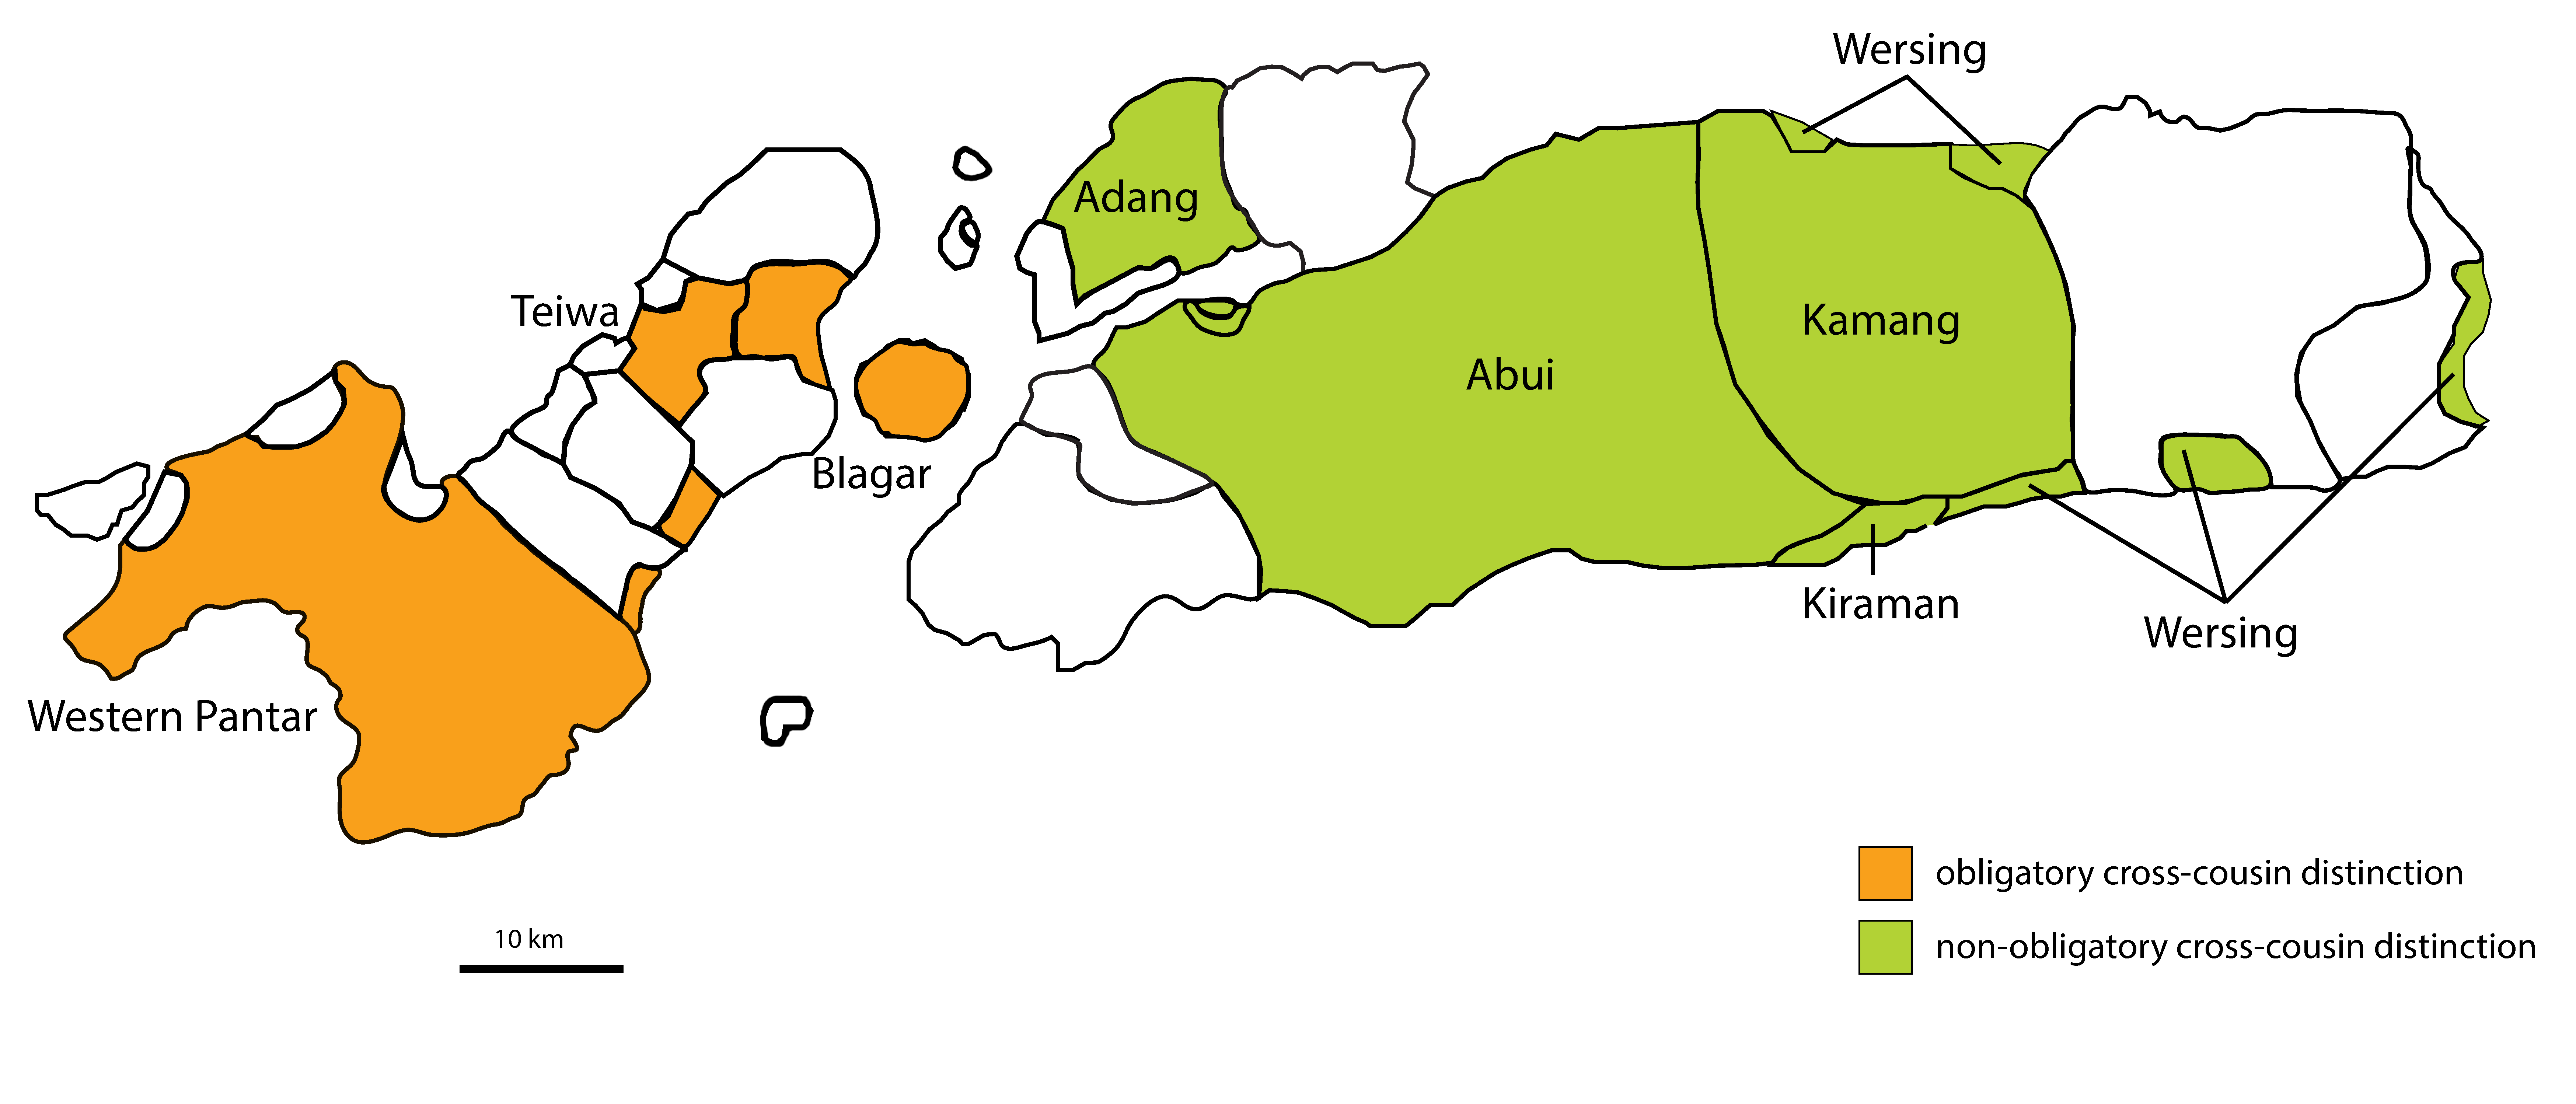
\includegraphics[width=\textwidth]{figures/Holton_ch5_fig15.pdf}
\caption{Geographic distribution of languages according to whether  cross-cousins are obligatorily distinguished}
\label{fig_cross-cousin_map}
\label{fig:5:15}
\end{figure}  
 

In contrast, those languages which obligatorily distinguish cross-cousins from siblings are restricted to Pantar and the neighboring small island of Pura. These are primarily coastal and lowland areas (or at least places with easy access to the coast) which would have had substantially more contact with Alorese\il{Alorese}, the language spoken by Austronesian\il{Austronesian language(s)} migrants who arrived in Alor during the last millennium \citep{Klamer2011}. In this context it is notable that Alorese\il{Alorese} has a symmetric alliance system which distinguishes cross-cousins from siblings \citep{Needham1956,Barnes1973}. In Alorese, classificatory same-sex siblings are distinguished by age: \textit{kakang} `elder (same-sex) sibling' versus \textit{aring} `younger (same-sex) sibling'; and classificatory opposite-sex siblings are distinguished for gender: \textit{nang} `woman's brother' versus \textit{bineng} `man's sister'. Both maternal and paternal cross-cousins are referred to as \textit{opung} and may be distinguished for gender: \textit{opung kafae} `female cross-cousin' versus \textit{opung kalake} `male cross-cousin'. Moreover, these cross-cousin terms are used for affine (in-law) relations as well, yielding equations characteristic of a symmetric system. For example, \textit{opung kalake} is both mother's brother and wife's father. The equation MB = WF implies that a man's wife must be his cross-cousin, since his mother's brother is the classificatory father of his wife. These same equations hold in Western Pantar\il{Western Pantar} and Teiwa\il{Teiwa}, though not in the other languages, which largely retain reflexes of the original pAP\il{proto-Alor-Pantar} affine term *dat (see Table \ref{tab:5:18}). This suggests that in Western Pantar and Teiwa\il{Teiwa} the original affine term has been replaced by the cross-cousin term under pressure from a shift to a symmetric alliance system. 



Marriage practices may also be a result of contact with Alorese\il{Alorese}. Preference for cross-cousin marriage is strongest among the westernmost languages Western Pantar, Teiwa, and Blagar\il{Blagar} -- i.e., those languages which have likely had the most contact with Alorese\il{Alorese}. The preference for cross-cousin marriage is strongest in Western Pantar, where the equation W = MBD = FZD holds, with the result that all marriages are treated as if they were between cross-cousins. At the other end of the spectrum, Kamang\il{Kamang} explicitly forbids marriage between cross-cousins. In the more remote regions of central Alor, people view the concept of cross-cousin marriage as a coastal practice, often choosing to refer to it by its local Malay\il{Malay} designation, \textit{lake ruma - bini ruma}, literally `house husband - house wife', rather than using equivalent terms from their own languages. Among Kamang speakers, where such marriages are explicitly forbidden, discussion of this relationship generated derisive laughter. Among Abui\il{Abui} speakers there is an attitude of ambivalence. One speaker noted that ``some people do that now, and the elders have seen that it is okay''. 

Further evidence that the preference for cross-cousin marriage is an innovation\is{innovation} comes from the prevalence of terms for spouse's  sibling which are distinct from terms for cross-cousin (see Table \ref{tab:5:18} above). In a system of direct exchange based on cross-cousin marriage we would expect cross-cousins to be equated with affines in ego's generation, for, in such a system, ego's spouse's sibling should also be a cross-cousin. Yet this equation again holds only in the westernmost languages, where obligatory cross-cousin distinctions have emerged. 

Taken together this evidence, while admittedly circumstantial, suggests that the Alor-Pantar kinship\is{kinship} system was originally non-prescriptive, with no distinctions between siblings and cousins. These systems then underwent drift toward prescriptive systems under influence of the Austronesian\il{Austronesian language(s)} migrants. Some evolved asymmetric systems with preference for maternal cross-cousin marriage; while others evolved symmetric systems. Whether or not this historical scenario is correct must await further data and analysis. In the meantime it can be hoped that the data presented here go some way toward providing a fuller picture of kinship terminology in Alor-Pantar. Whatever the exact nature of proto-Alor-Pantar\il{proto-Alor-Pantar} kinship may have been, it is clear that the family today shows enormous variation in both kinship terminology and practice, in spite of the fact that the various language communities are closely bound together through ties of marriage alliance. The Alor-Pantar languages thus provide fertile ground for the investigation of the ways kinship systems may evolve.

\section*{Sources}
Data sources are as follows. Western Pantar\il{Western Pantar} is based on the author's own field work, primarily in 2007. Teiwa\il{Teiwa} is based on \citet{Klamer2010grammar} and field work by Laura C. Robinson in 2010 and 2011 and by the author in 2013. Blagar\il{Blagar} is based on published data in \citet{Steinhauer1993} as well as field work by Robinson in 2011. Kiraman\il{Kiraman} is based on the author's field work in 2010 and 2013. Adang\il{Adang} is based on field work by Robinson in 2010 and 2011 and by the author in 2013. Abui\il{Abui} is based on \citet{KratochvilEtAl2008kamus} and field work by the author in 2013. Kamang\il{Kamang} is based on \citet{Stokhof1977}, \citet{SchapperEtAl2011kamus}, and the author's field work in 2010 and 2013. Wersing\il{Wersing} is based on the author's work in 2010 and 2013. Alorese\il{Alorese} (Austronesian\il{Austronesian language(s)}) is based on \citet{Needham1956} and \citet{Barnes1973}. The author has conducted primary field work with all languages discussed in this chapter except Blagar\il{Blagar}, and in all cases the author accepts full responsibility for any errors of fact or interpretation.

\section*{Acknowledgments}
I wish to acknowledge the many speakers who assisted with research on kinship\is{kinship} terms in Alor-Pantar languages, especially: Mahalalel Lamma Koly, Nathan Lamma Koly, Amos Sir, Yarid Malaimakuni, Marlon Adang, Benny Delpada, Yulius Mantaun, Agus Mantaun and Ans Retebana, among many others. I also thank Marian Klamer, James Fox, and Hein Steinhauer for their critical comments on an earlier draft of this chapter.


\section*{Abbreviations}


\begin{tabular}{ll}
B & brother\\
C & child\\
D & daughter\\
e & elder\\
F & father\\
f & woman  speaking\\
H & husband\\
M & mother\\
m & man speaking\\
S & son\\
W & wife\\
y & younger\\
Z & sister\\
\end{tabular}

